
\documentclass[12pt,a4paper,twoside]{report}
\usepackage[pdfborder={0 0 0}]{hyperref}    % turns references into hyperlinks
\usepackage[margin=20mm]{geometry}  % adjusts page layout
\usepackage{graphicx}  % allows inclusion of PDF, PNG and JPG images
\graphicspath{ {./images/} }
\usepackage{verbatim}
\usepackage{amsmath}
\usepackage{amssymb}
\usepackage{dirtree}
\usepackage{mathtools}
\DeclarePairedDelimiter\paren{\lparen}{\rparen}
\DeclarePairedDelimiter\bracks{\lbrack}{\rbrack}
\usepackage{xcolor}
\usepackage{tikz}
\usetikzlibrary{arrows,positioning,shapes.geometric}
\usepackage[edges]{forest}
\usepackage{algorithm}
\usepackage[noend]{algpseudocode}
\usepackage{docmute}   % only needed to allow inclusion of proposal.tex
\usepackage{neuralnetwork}
\usepackage{adjustbox}

\raggedbottom                           % try to avoid widows and orphans
\sloppy
\clubpenalty1000%
\widowpenalty1000%
\setcounter{secnumdepth}{4}
\setcounter{tocdepth}{4}

\renewcommand{\baselinestretch}{1.1}    % adjust line spacing to make
                                        % more readable

\begin{document}

%%%%%%%%%%%%%%%%%%%%%%%%%%%%%%%%%%%%%%%%%%%%%%%%%%%%%%%%%%%%%%%%%%%%%%%%
% Title

\pagestyle{empty}

\rightline{\LARGE \textbf{Manu Varma}}

\vspace*{60mm}
\begin{center}
\Huge
\textbf{Kin Recognition Using Weighted Graph Embeddings} \\[5mm]
Computer Science Tripos -- Part II \\[5mm]
St John's College \\[5mm]
\today  % today's date
\end{center}

%%%%%%%%%%%%%%%%%%%%%%%%%%%%%%%%%%%%%%%%%%%%%%%%%%%%%%%%%%%%%%%%%%%%%%%%%%%%%%
% Proforma, table of contents and list of figures
\let\cleardoublepage\clearpage
\pagestyle{plain}

\newpage
\section*{Declaration}

I, Manu Varma of St. John's College, being a candidate for Part II of the Computer
Science Tripos, hereby declare
that this dissertation and the work described in it are my own work,
unaided except as may be specified below, and that the dissertation
does not contain material that has already been used to any substantial
extent for a comparable purpose.

\bigskip
\leftline{Signed Manu Varma}

\medskip
\leftline{Date \today}

\chapter*{Proforma}

{\large
\begin{tabular}{ll}
Candidate Number:   & \bf 2356E                       \\
Project Title:      & \bf Kin Recognition Using Weighted \\ & \bf Graph Embeddings \\
Examination:        & \bf Computer Science Tripos -- Part II, June 2021  \\
Word Count:         & \bf TBA  \\ % TODO: Change
Line Count:         & \bf 3027 \footnote{Calculated using \texttt{find . -name '*.py' | xargs wc -l}}  \\ % TODO: Change
Project Originator: & \bf The Dissertation Author                   \\
Supervisor:         & \bf Daniel Bates                    \\ 
\end{tabular}
}
\section*{Original Aims of the Project}

\section*{Work Completed}

\section*{Special Difficulties}
None.

\tableofcontents

\listoffigures


\pagestyle{headings}

%%%%%%%%%%%%%%%%%%%%%%%%%%%%%%%%%%%%
%%%%%%%%%%% Introduction %%%%%%%%%%%
%%%%%%%%%%%%%%%%%%%%%%%%%%%%%%%%%%%%

\chapter{Introduction}
% TODO: A stronger hook sentence is definitely needed here. 

Kinship recognition is the ability to recognize how two people are related to each other based on how their faces. This is an evolutionary trait in humans as it is advantageous to inclusive fitness for an organism to be able to recognize which of their neighbors are close relatives \cite{HamiltonGenetic}. Thus, it stands to reason that the ability to recognize kinship relationships has evolved in humans. 
In humans, specifically, facial resemblance is expected to serve as an indicator of kinship as we have seen that strangers are able to match photographs of mothers to their infants without any prior contact with any of the family \cite{mateo2015}. 

Computational kinship recognition is the field of computationally figuring out kinship relationships between people without any prior knowledge of the family. 

\section{Problem Overview}

There are multiple problems in the field of computational kin recognition, and I will focus on solving one of them. The first of which takes as input a pair of images and a proposed kinship relationship, for example mother-daughter, and recognizes whether the relationship exists. We can see an example set of images in figure \ref{fig:KinRecogEx}.

\begin{figure}[!ht]
    \centering
    \includegraphics{Intro/face_example.png}
    \caption{An example of an input into a classical kin recognition problem}
    \label{fig:KinRecogEx}
\end{figure}

These relationships tend to be more commonly parent-child relationships as opposed to sibling-sibling relationships, for example. A further extension of the main kin recognition problem is Tri-Subject Kinship which takes 3 images, two parents and a child, and determines if they are related 
or not. These problems are the ones that are being looked at in this dissertation. 

Some other major problems in the field include search-and-retrieval and family classification. Search-and-retrieval is the problem which takes an image of a person as input and searches through a database to find people with whom they are most likely to be related to. This outputs a list of these people that they could be related to. 
Family classification deals with a similar task of taking an image of a person as input and figuring out which family they may belong to. 

\section{Motivation}

Accurate kinship recognition software has multiple applications in humanitarian issues. 
With regards to humanitarian issues, by using kin recognition, we can better recognize missing children and match them with their parents \cite{robinson2020visual}.
It can also be used for stopping human traffickers from claiming they are family members of the victim or to reunite families across refugee camps. 

Furthermore, there are potential use-cases in social media and it can also pose privacy protections. % ??????
% TODO: Strengthen up the motivations here 
\section{Related Work}     

One of the first papers in the field of computational kinship recognition used color, facial parts, facial distances and a Histogram of Gradients vector as the features for each image. 
Using these features, K-Nearest-Neighbors and a Support Vector Machine (SVM) were used in order to classify the image pairs into true and false parent-child pairs \cite{fang2010}. A classification accuracy of $70.67\%$ was obtained overall and an SVM with a radial basis kernel obtained an accuracy of $68.6\%$. 

Other approaches include using deep learning to solve the problem. One paper used a Siamese Convolutional Neural Network (CNN) approach by putting both of the face images in the pair through a SqueezeNet network which was trained on VGGFace2 which creates a feature vector for each image \cite{DeepSiameseCNN}. Using a similarity criterion, a new feature vector is created using the two feature vectors and a fully connected layer and a sigmoid activation function creates the predicted similarity score. This approach yielded an average test accuracy of $67.66\%$ over all of the relationships that were in the dataset. 
Another paper that used a Siamese approach aimed to solve both the standard kinship verification problem and the Tri-Subject problem \cite{DeepFusion}. Both networks for the problems had three stages, a feature extraction stage, which used the ResNet50 or SENet50 models pre-trained on VGGFace2 to extract the features from each face into a vector, a feature fusion stage which combines the feature vectors together, and a similarity quantization stage to get the similarity score. 
They then use a jury system to fuse together models which allows them to achieve an accuracy of $75.9\%$. 

However, a prominent approach that is taken includes using metric learning to solve the problem. For example, the paper on Neighborhood Repulsed Metric Learning \cite{KinFaceCitation1} uses a supervised metric learning approach. Using the approach, they aim to find a metric which minimizes the distance between the vectors of images that have a kinship relationship and maximize the distances between the vectors of pairs of images that don't have a kinship relationship. 
Furthermore, the paper that will be implemented in this dissertation, using Weighted Graph Embedding-Based Metric Learning, involves a metric learning approach to the problem \cite{WGEML}. 

\section{Project Overview}

The project aims to reproduce the results of the paper, Weighted Graph Embedding-Based Metric Learning \cite{WGEML}, or WGEML for short, and aims to implement the paper and verify the accuracies that were obtained. 
The following is shown in the dissertation:

\begin{enumerate}
    \item The algorithm, WGEML, is implemented and accuracies that are within an acceptable range are obtained, as shown in section \ref{sec:MainResults}.
    \item Ablation studies on the face descriptors are performed and the results are in section \ref{sec:FDAbStudies}.
    \item We use the models that were created to discover biases in the datasets that were used and find out the impact that has overall in section \ref{sec:Biases}. 
    \item We further test the face descriptors by replacing VGG with a smaller CNN in which the implementation is discussed in section \ref{sec:CFNExt}. 
\end{enumerate}

Chapter \ref{chapter:Prep} explains much of the needed technical background for the implementation, from what a Neural Network is and what metric learning is to each of the face descriptors used and what face descriptors are. 
Chapter \ref{chapter:Implementation} will then discuss the specifics of how WGEML and the extension that used a different network than VGG was implemented. 
Chapter \ref{chapter:Evaluation} then discusses all of the results that were obtained from experimentation with WGEML and the implications of the results. 

%%%%%%%%%%%%%%%%%%%%%%%%%%%%%%%%%%%
%%%%%%%%%%% Preparation %%%%%%%%%%%
%%%%%%%%%%%%%%%%%%%%%%%%%%%%%%%%%%%

\chapter{Preparation} \label{chapter:Prep}

In this chapter, I discuss the necessary technical background information needed for the project in sections \ref{sec:CNN} through \ref{sec:KNN}, then the requirements of the project are elaborated on in section \ref{sec:ReqAnal} before the starting point and Software Engineering practices are discussed in section \ref{sec:SEPractices}. 

\section{Convolutional Neural Networks} \label{sec:CNN}

To talk about Convolutional Neural Networks, first we must discuss what an artificial neural network (ANN) is. An ANN is a collection of connected nodes. These are organized into layers such that there is an input and output layer as well as multiple layers in between which do some computation. The layers are made up of the connected nodes. 

A basic type of this is a Multilayer Perceptron (MLP) which is a set of layers like we see in figure \ref{fig:ANNEx} which have neurons in each of the layers which each output one value. 

\begin{figure}[ht]
    \centering
    \begin{neuralnetwork}[height=4]
        \newcommand{\x}[2]{$x_#2$}
        \newcommand{\y}[2]{$\hat{y}_#2$}
        \newcommand{\hfirst}[2]{\small $h^{(1)}_#2$}
        \newcommand{\hsecond}[2]{\small $h^{(2)}_#2$}
        \inputlayer[count=3, bias=true, title=Input\\layer, text=\x]
        \hiddenlayer[count=3, bias=false, title=Hidden\\layer 1, text=\hfirst] \linklayers
        \hiddenlayer[count=3, bias=false, title=Hidden\\layer 2, text=\hsecond] \linklayers
        \outputlayer[count=2, title=Output\\layer, text=\y] \linklayers
    \end{neuralnetwork}
    \caption{An example of an artificial neural network with two hidden layers}
    \label{fig:ANNEx}
\end{figure}

If we have that $\mathbf{x}$ is the input layer, $\mathbf{h_i}$ is the $i$th hidden layer and $\mathbf{y}$ is the output layer, then an MLP can be written as:

\begin{align*}
    \mathbf{h_1} &= f_1(\mathbf{W_1}\mathbf{x} + \mathbf{b_1}) \\
    \mathbf{h_2} &= f_2(\mathbf{W_2}\mathbf{h_i} + \mathbf{b_2}) \\
    ... &= ... \\
    \mathbf{h_i} &= f_i(\mathbf{W_i}\mathbf{h_{i - 1}} + \mathbf{b_i}) \\
    ... &= ... \\
    \mathbf{y} &= f_{n + 1}(\mathbf{W_{n + 1}}\mathbf{h_n} + \mathbf{b_{n + 1}})
\end{align*}

Where $f_i$ represents the activation function for the corresponding layer and $\mathbf{W_i}$ and $\mathbf{b_i}$ are the weights and biases for the $i$th hidden layer which are the trainable parameters and $n$ is the number of hidden layers. 

A Convolutional Neural Network (CNN) is a type of neural network which is used to process data with a grid pattern which have some spatial locality, such as images. As opposed to an artificial neural network which is just composed of fully-connected layers, a CNN also uses convolutional layers and pooling layers \cite{CNN1}. Fully-connected layers have it so that each neuron in the layer have all of the connections to each of the input values, which is the same as in regular neural networks. 

\subsection{Convolutional Layers}

A convolutional layer takes an input image and, as hyperparameters, takes the number of output filters, kernel size and stride size in order to create a set of kernels and biases in order to create the output. 
A kernel is a matrix which is usually small and has sizes less than that of the input image but covers the depth of the entire input image. So, for example, if the input to a convolutional layer was $32 \times 32 \times 64$, then a kernel could have size $3 \times 3 \times 64$ where the first two sizes are specified. 
The kernel is then started in the top left of the input and the dot product of the kernel and the input sub-array is taken to be the output at that cell. An illustration of this is seen in figure \ref{fig:ConvLayer}.

\begin{figure}[h!]
    \centering
    \includegraphics[scale=0.5]{Prep/Convolution.png}
    \caption{A convolution done on an input. Image sourced from Yakura et al. (2018) \cite{CNNFigure}}
    \label{fig:ConvLayer}
\end{figure}

Then the kernel is moved along as much as specified in the stride. So, if the stride was $2 \times 2$, then the kernel would move 2 to the right and do the same thing. 

However, this produces a 2-dimensional array whereas we want a 3-dimensional volume as the output with a certain specified depth, which is the number of output filters. Thus, that many kernels are created and used for the layer to create the output. These 2-dimensional arrays are then stacked on top of each other to create a 3-dimensional output. 
A bias is then applied and the activation function is applied to the output, which is usually ReLU which is described in section \ref{sec:ReLU}. 

\subsection{Pooling Layers}

Pooling layers in a CNN tend to reduce the dimension of the representation which, in turn, reduces the size of the representation. 
There are multiple pooling layer types, such as max-pooling and average-pooling, which are the two types that are used in this project in VGG and CifarNet which are discussed in sections \ref{sec:VGGPrep} and \ref{sec:CFNExt}. 
These pooling layers take an input of size $W_1 \times H_1 \times D_1$, have hyperparameters which are the stride, $S$, and filter size, $F$, and output a tensor of size:

\[\frac{W_1 - F}{S + 1} \times \frac{H_1 - F}{S + 1} \times D_1\]

This output is calculated by taking each $F \times F$ subarray for each slice of the input and doing the corresponding operation on it and returning that as the output for that cell. So, max-pooling would take the max of each of the $F \times F$ cells and average-pooling would take the average. The stride is the same as the stride in the convolutional layer.
We can see an example of this with a max pooling layer of stride 2 and has filter size $2 \times 2$ in figure \ref{fig:PoolEx}.

\begin{figure}[h!]
    \centering
    \includegraphics[scale=0.5]{Prep/poolingExample.jpeg}
    \caption{An example of the max pooling operation done on a single slice of the input}
    \label{fig:PoolEx}
\end{figure}

\subsection{Activation Functions}

There are a multitude of functions which are applied to the output of a layer which have different effects. These are called activation functions and we'll talk about two of them here, ReLU and Softmax. Only nonlinear activation functions are considered due to the fact that we want to be able to have nonlinear decision boundaries. If we had linear activation functions, the neural network would still be linear in nature and, thus, we wouldn't be able to deal with non-linear problems. 

\subsubsection{ReLU} \label{sec:ReLU}

ReLU applies the following on each output of a layer:

\[f(x) = \max(0, x)\]

In other words, it makes sure that all negative values become 0. This is simple to calculate and has the property that the derivative is either 1 or 0 which makes the gradient computation simpler. Due to the simplicity of the activation function, this helps speed up training a neural network. 

\subsubsection{Softmax}

Another one is the softmax function which takes a vector, $\mathbf{z}$ and the component-wise output is:

\[\sigma(\mathbf{z})_i = \frac{e^{z_i}}{\sum_{j = 1}^{N} e^{z_j}}\]

Where $N$ is the dimension of the input vector. In other words, it takes a vector and outputs a vector of the same size where the sum of the values of the vector adds up to 1, so you can interpret the individual values as probabilities. This is a useful activation function for the last layer of a neural network that solves a classification problem. For example, in the CifarNet model in section \ref{sec:CFNExt}, the last layer has the softmax function applied to it in order for each of the 10 values to be interpreted as a probability that the input image was the corresponding class. 

\section{Face Detection} \label{sec:FaceDetection}

Face detection is the task of finding faces within a given image and returning the set of faces found. 
This differs from face recognition since the task is only to find the faces and not to recognize who the faces belong to. The project uses OpenCV's version of face detection which is a cascade classifier and is discussed in appendix \ref{sec:Cascade}. 

\section{Face Descriptors} \label{sec:PrepFD}

We wish to be able to create a mapping from a colored image into a vector to make computations easier and to be able to determine similarity between images. These are called image descriptors for general images. When we try and map face images to vectors, we call these face descriptors. 
We want these face descriptor mappings to be able to match the same person in different poses and illuminant geometries to face descriptors that are close to each other in distance. Thus, these mappings try and capture color, texture, and shapes,
for example. There are multiple face descriptors that can be made of a face image, each of which extracts different features from the face. We use the Local Binary Patterns, Histogram of Gradients, Scale-Invariant Feature Transform and VGG face descriptors to extract features from each face.

\subsection{Local Binary Patterns}

The Local Binary Patterns (LBP) visual descriptor which is adapted for faces is a texture descriptor \cite{LBPFace} which means that the algorithm attempts to describe the texture of the image, rather than anything to do with the color. 
As such, given an image, we must first convert it to grayscale. This can be done in various ways but in the project, the OpenCV method is used which maps each RGB pixel to the grayscale value\footnote{Information taken from \url{https://docs.opencv.org/3.4/de/d25/imgproc_color_conversions.html} using the RGB to Gray color conversion}:

\[0.299\times R+0.587\times G+0.114\times B\]

Then, for each pixel in the image, a neighborhood of pixels is obtained from it. There are multiple ways to define this neighborhood, as shown in figure \ref{fig:LBPNeighborhood}. 

\begin{figure}[ht]
    \centering
    \includegraphics[scale=0.2]{Prep/Lbp_neighbors.png}
    \caption{Potential neighborhoods of the pixel}
    \label{fig:LBPNeighborhood}
\end{figure}

The simplest neighborhood, which is the neighborhood used in this project, is the direct neighbors of the pixel, which is the first neighborhood in figure \ref{fig:LBPNeighborhood}. 
However, on the edges, some of the neighbors won't exist. To mitigate this, in the implementation, I pad the grayscale image with 0s on the outside of the image such that each pixel in the image has the same number of neighbors. 
Once we have our neighborhood of the pixel, we compare the grayscale value of the main pixel with each of the grayscale values in the neighborhood. For each neighboring value, if it is greater than the main pixel, we make it a $1$, otherwise we make it a $0$. 
We are then able to create a binary number from the neighboring values. In practice, where the number is started from doesn't matter but in my implementation, the number starts from the left cell and goes counterclockwise. 
Applying this to figure \ref{fig:LBPExample}, we get that our LBP value for this pixel would be $01111000_2$ which, in decimal, is $120$. 

\begin{figure}[ht]
    \centering
    \includegraphics[scale=0.75]{Prep/LBPExample.png}
    \caption{Example of LBP operator on a pixel}
    \label{fig:LBPExample}
\end{figure}

To summarize the LBP operator mathematically, given a coordinate in the image, $(x, y)$ which has grayscale value $g$, a neighborhood of $P$ points with radius $R$ enumerated by $g_p$ where $p \in \{0, P - 1\}$, we have that \cite{textureSurvey}:
\[LBP_{P, R}(x, y) = \sum_{p = 0}^{P - 1} s(g_p - g)2^p\]
Where:
\[s(x) = \begin{cases} 1 & \text{if } x > 0 \\ 0 & \text{else} \end{cases}\]

Once we get the values of the pixel, an added extension, which we do for face description, is to check whether it is a \textit{uniform value} which we define as a value such that, in binary, there are only, at most, 2 bitwise transitions when traversed circularly. For example, 11000111 is a uniform value since it only transitions from 1 to 0 and 0 to 1 but 11001000 isn't since it has 4 bitwise transitions. 
With this extension, we have 58 possible uniform values that a pixel's LBP value can be and an extra value for the LBP value not being uniform. In other words, there are 59 LBP values that a pixel in an image can take. 

Once each pixel in the image has an associated LBP value, we can split up the image into blocks. For our implementation, since our input images have size $64 \times 64$, we split it up into non-overlapping blocks of size $8 \times 8$, of which there are $8 \times 8$. 
For each block, we obtain a histogram of the LBP values that were in the block, which gives us a $59$-dimensional vector. To obtain the vector for the entire image, each of these vectors are appended together and a 3776-dimensional LBP face descriptor is obtained for our case. 

\subsection{Histogram of Gradients}\label{sec:HOG}

Another face descriptor is Histogram of Gradients (HOG) \cite{HOG}. Given a colored image, we can think of the image as a function, $I: \mathbb{N}_m \times \mathbb{N}_n \to \mathbb{R}^3$, which takes a coordinate in the image and returns a vector of values, which correspond to the red, green, and blue values of the pixel.
This then means that we are able to calculate the gradient of the image. The gradient of an image can characterize local object appearance and shape due to the fact that the gradient of the image can be used to help find edges in the image. As such, it is useful to obtain such a histogram of gradients. 

\subsubsection{Calculating the Gradients}

First, we need to calculate the gradients of the image. As the image function is discrete, in other words we cannot analytically find the gradients, we must find approximations to do so. This is done by convolving specific kernels on the image. 
What this means is that the kernel, $K$ which is a matrix, is applied to each pixel in the image and its neighbors and the values are multiplied with the corresponding value in the kernel and all of the values are then summed up to create the new value for the convolved image. 
For example, if we had the kernel:

\[K = \begin{bmatrix}
    1 & 2 & 1
\end{bmatrix}\]

And the image:
\[I = \begin{bmatrix}
    0 & 5 & 4 \\ 3 & 3 & 3 \\ 2 & 1 & 2
\end{bmatrix}\]

We get that the kernel convolved on the image is:
\[K * I = \begin{bmatrix}
    0\times 1 + 5\times 2 + 4\times 1 \\
    3\times 1 + 3\times 2 + 3\times 1 \\
    2\times 1 + 1\times 2 + 2\times 1 
\end{bmatrix} = \begin{bmatrix}
    14 \\
    12 \\
    6
\end{bmatrix}\]

We can then approximate the derivative of an image using a kernel being convolved on the image. To do so, we use the kernels:
\begin{align*}
    G_x &= \begin{bmatrix} -1 & 0 & 1\end{bmatrix} \\
    G_y &= \begin{bmatrix} -1 & 0 & 1\end{bmatrix}^T
\end{align*}

By convolving these kernels on the image, we are able to get an estimate for the derivative in the $x$ direction and in the $y$ direction, respectively. 
Abusing notation slightly where here the square of the matrix just means an element-wise square and division just means element-wise division, we get that the magnitude of the gradient is:

\[\sqrt{(G_x * I)^2 + (G_y * I)^2}\]

And that the angles at each point are:

\[\tan^{-1}((G_y * I)/(G_x * I))\]

However, there are two things that need to be addressed before we move on to the rest of the algorithm. Firstly, there are still 3 channels for the image, so we have obtained the gradient in the $x$ and $y$ direction for each pixel and each channel. As such, 
we define the gradient of each pixel to be the gradient which has the maximum magnitude among the 3 channels and the corresponding angle is used as well. 

Furthermore, the angles returned range between $0^{\circ}$ and $360^{\circ}$. However, we require that the angles be ``unsigned'', so the angle at each pixel, $\theta_{(x, y)}$, becomes:

\begin{center}
\texttt{$\theta_{(x, y)}$ := $\theta_{(x, y)}\mod{180}$}
\end{center}

\subsubsection{Weighted Vote into Histogram}

At this point, we have the magnitude of the gradient at each point in the image as well as the angle of the gradient. Now, similarly to LBP, we break up the image into blocks. 
We create a histogram for each of these blocks and append them together to make the face descriptor for the entire image. 
Unlike LBP however, we don't have a finite set of labels that each pixel can neatly fall into however, since neither the magnitude nor the angles are discrete. Thus, first, the labels of the histogram are going to be the angles of the gradients. 
The labels will then be:
\[[0, 20, 40, 60, 80, 100, 120, 140, 160]\]
However, these aren't blocks ranges of $[0, 20)$, for example. Instead, for each pixel in the block, we distribute the magnitude of the gradient of the pixel between the angles that the angle falls between. 
Given a pixel with magnitude $m$ and angle $\theta$, if $0 \equiv \theta \mod{20}$ then:

\begin{center}
    \texttt{histogram[$\theta/20$] += $m$}    
\end{center}

Otherwise, we have it that $\theta$ is between two angles, $\phi_1$ and $\phi_2$, both of which are divisible by $20$, where $\phi_1 < \theta < \phi_2$. 
In this case, we weight the amount that we add to each label based on how far away $\theta$ is to the label. So, for the label $\phi_1$, we have that we add to the label associated with $\phi_1$ the value:

\[\frac{\phi_2 - \theta}{20} \times m\]

And, similarly for $\phi_2$:

\[\frac{\theta - \phi_1}{20} \times m\]

In other words, the closer the angle is to the label, the more of the magnitude is contributed to the label's histogram value. As a caveat, if $\phi_2 = 180^{\circ}$, we treat $\phi_2$ as $180^{\circ}$ for the sake of this calculation but we add the value to the label $0$ since $0 \equiv 180 \mod{180}$. 

We can do this for each pixel in the block and, thus, we are able to get a $9$-dimensional vector for each block. 
In the project, the image is split up into $16 \times 16$ blocks of size $4 \times 4$ first and then $8 \times 8$ blocks of size $8 \times 8$ next and each of these blocks contributes a histogram to the overall vector which leads us with a face descriptor with dimension:
\[16 \times 16 \times 9 + 8 \times 8 \times 9 = 2880\]

\subsection{Scale-Invariant Feature Transform} \label{sec:SIFTPrep}

SIFT \cite{SIFT} is another way of obtaining face descriptors, although the original SIFT algorithm differs from how it is used in the project,. The algorithm, generally, is split into finding the keypoints, fine tuning the keypoints, assigning an orientation to each keypoint and then getting a descriptor from each keypoint. The method of obtaining each of the keypoints in an image, which are just points of interest which can be near important features of the image, is explained in Appendix \ref{sec:AppendixSIFT}.

Once we have the keypoints in the image, a $16 \times 16$ window is obtained around the keypoint and divided into 16 blocks. For each block, a histogram of the gradients is taken with 8 bins which are then appended together which gives a 128-dimensional vector for the keypoint. The SIFT descriptor of the image is then the vectors for each keypoint appended together to create a $128n$-dimensional vector where $n$ is the number of keypoints in the image. 

The actual implementation of SIFT that is used differs from the original version which is talked about in section \ref{sec:SIFTImpl}.

\subsection{VGG} \label{sec:VGGPrep}

Another way of getting face descriptors for an image is to use the VGG network. The original VGG network \cite{VGG} is a CNN which takes in a $224 \times 224$ colored image and outputs a probability vector of size 1000 for the ImageNet classes. In other words, if \texttt{out} is the output of the model, \texttt{out[i]} corresponds with the probability that the \texttt{i}$^{\text{th}}$ ImageNet class is the class of the input image. 
There are 5 configurations of the network, which have varying depth and, as a result, more parameters. The architecture of the second deepest configuration is configuration D in Figure \ref{fig:VGGArch}.

\begin{figure}[ht]
    \centering
    \includegraphics[scale=0.65]{Prep/VGGArch.png} 
    \caption{The different configurations that VGG can have. Image reproduced from Simonyan et al. (2015) \cite{VGG}}
    \label{fig:VGGArch}
\end{figure}

By training this model on the ImageNet dataset, the model is able to get a top-5 classification error of 7.5\%, which means that for 7.5\% of the entries in the test set, none of the top 5 classes that the image could be were the actual image. 

However, in order to use the model for face description, we must change the output layer and the training dataset \cite{VGGFace}. Instead of training on general objects in an image, we train the model on faces, specifically celebrity faces. 
The celebrities are curated to a list of 2622 people in which 2000 images are obtained for each celebrity and the images are then curated. The curated set of images constitutes the training set for the VGG model for faces. This dataset\footnote{The dataset is available at \url{https://www.robots.ox.ac.uk/~vgg/data/vgg_face/}} was created by the authors of \cite{VGGFace}.

The VGG model for faces is then the model described above with the softmax layer having dimension of 2622. The model is then trained with the dataset we described which allows us to get rid of the softmax layer and use the output of the last fully-connected layer as our 4096-dimensional face descriptor for the image. 

\section{Metric Learning} \label{sec:MetricLearningPrimer}

We wish to measure the similarity between a pair of faces in order to determine whether they are related or not. One way to approach this is to use similarity learning in which the goal is to learn a similarity function in order to measure how similar two objects are. 
However, we often use distance to help measure the similarity between data points. By learning what this distance function ought to be, we would be able to find a better similarity function so finding this distance function is the goal of metric learning \cite{metricLearningPrimer}. To go more in depth, we must first define a few concepts.

Given a non-empty set $A$, we define a \textit{distance} over $A$ as a function $d: A \times A \to \mathbb{R}$ such that the following holds:
\begin{enumerate}
    \item \textbf{Non-Negativity}: $\forall x, y \in A$, $d(x, y) \geq 0$ 
    \item \textbf{Coincidence}: $\forall x, y \in A$, $d(x, y) = 0$ if and only if $x = y$. 
    \item \textbf{Symmetry}: $\forall x, y \in A$, $d(x, y) = d(y, x)$
    \item \textbf{Triangle Inequality}: The triangle inequality must hold. That is, $\forall x, y, z \in A$: 
    \[d(x, y) + d(y, z) \geq d(x, z)\]
\end{enumerate}

Given the definition of a distance, we define a \textit{Mahalanobis distance} that corresponds to the positive semidefinite matrix $M$ to be a distance function, $d_M: \mathbb{R}^d \times \mathbb{R}^d \to \mathbb{R}$, where $d$ is the number of dimensions the input vector has which is defined as:
\[d_M(x, y) = \sqrt{(x - y)^TM(x - y)}\]

If $M$ is positive semidefinite, then $M$ must be decomposable into $B^TB$ where $B$ is a real matrix. Thus, we can also write the Mahalanobis distance as:
\[d_M(x, y) = \sqrt{(x - y)^TM(x - y)} = \sqrt{(x - y)^TB^TB(x - y)} = \sqrt{(Bx - By)^T(Bx - By)}\]

So the Mahalanobis distance is essentially a Euclidean distance after applying a linear transformation to each of the input vectors. 
This makes it so that we only have to learn what this linear transformation is which is simpler to find than searching through the set of all possible distance functions to see which is the best overall. 

The Mahalanobis distance is a \textit{pseudometric}, which is a distance function in which the coincidence property doesn't hold, when the matrix $M$ isn't full-rank. A matrix is \textit{full-rank} when the rank of the matrix is either equal to the number of rows or columns in the matrix.

Thus, given a dataset $\mathcal{X} = \{x_1, ..., x_n\} \subset \mathbb{R}^d$ which has the sets:

\[S = \{(x_i, x_j) \in \mathcal{X} \times \mathcal{X} \mid x_i \text{ and } x_j \text{ are similar}\}\]
\[D = \{(x_i, x_j) \in \mathcal{X} \times \mathcal{X} \mid x_i \text{ and } x_j \text{ are not similar}\}\]

We wish to find the distance metric $M$ such that we can minimize some loss function, $l$:
\[\min_{M} l(d_M, S, D)\]

In other words, in metric learning, we wish to find out what the matrix $M$ should be defined as in order to make data points which are similar closer together and data points which aren't similar further away, which is encapsulated by the loss function. 
We can visualize this in figure \ref{fig:MetricLearning}.

\begin{figure}[ht]
    \centering
    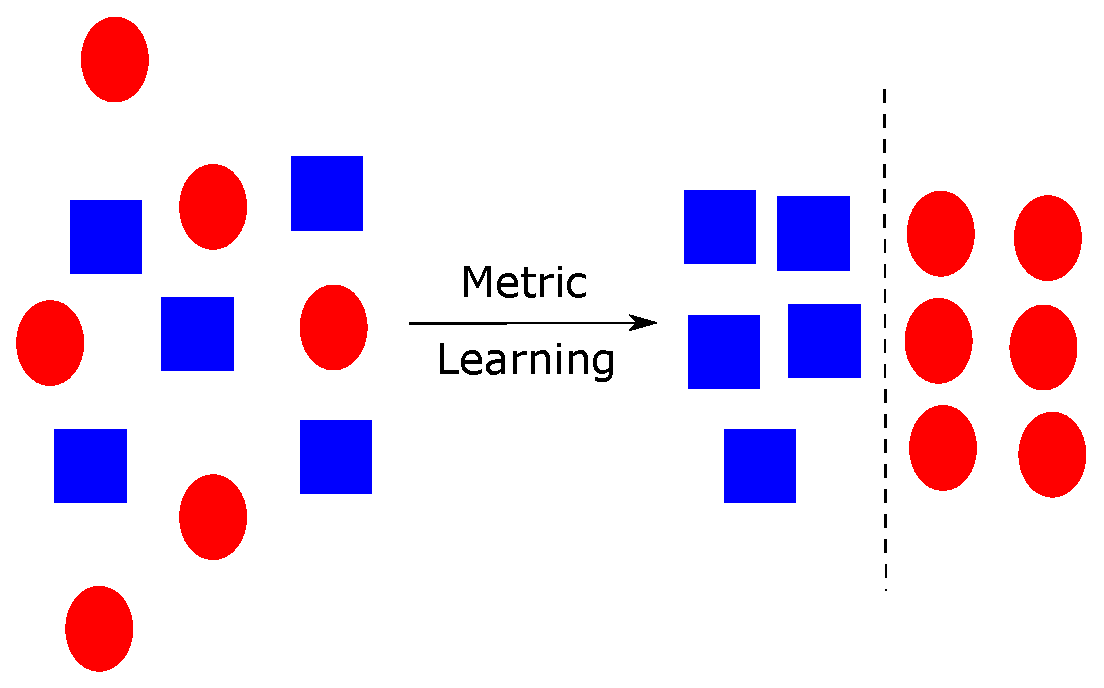
\includegraphics[scale=0.65]{Prep/MetricLearningEx.eps}
    \caption{A high-level view of metric learning}
    \label{fig:MetricLearning}
\end{figure}

\section{K-Nearest Neighbors} \label{sec:KNN}

K-Nearest Neighbors is an algorithm that finds the $K$ nearest neighbors for each datum in a given set of data. Given a list of datapoints in Euclidean space, we wish to find, for each datapoint, the $K$ closest datapoints to it. The \texttt{sklearn} library is used to implement it which uses a brute force algorithm, a ball tree or a $kd$-tree depending on the input.

\section{Requirements Analysis} \label{sec:ReqAnal}

The main requirement of the project is stated in appendix \ref{chapter:Proposal} which is to replicate the results from Liang et al. (2019) \cite{WGEML} within a $15\%$ error range or to reject the results. In other words, the project should implement the Weighted Graph Embedding-Based Metric Learning (WGEML) algorithm for Kin Recognition. 
The core project can be broken down into the following requirements:
\begin{itemize}
    \item \textbf{Face Detection}: Given an image, the faces in the image must be identified and saved as a $64 \times 64$ image on disk. 
    \item \textbf{Face Descriptors}: The face descriptors, LBP, HOG, SIFT and VGG, must be implemented such that, given an image, each of these face descriptors should be able to be obtained from them. 
    \item \textbf{WGEML}: The WGEML algorithm must be implemented such that, given a relationship, the positive pairs of faces, the negative pairs of faces, if any, it returns the distance metric matrix for each face descriptor used and how much each face descriptor should be weighted in the prediction step. 
    \item \textbf{Prediction}: Given the model obtained from the WGEML algorithm, a pair of images, and a relationship, it must return how similar the images are and whether the people in the images have the kin relationship given. 
    \item \textbf{End-to-end Replication}: Running the project end-to-end on the given datasets either gives similar results to the original paper or rejects the original results. 
\end{itemize}

The extensions can be summarized as follows:
\begin{itemize}
    \item Replace the VGG face descriptor with a smaller network to see how it affects accuracies. 
    \item Look at how biases in the datasets affect the results and identify these biases. 
    \item Use different combinations of face descriptors for WGEML to see how it affects accuracy of the model. 
\end{itemize}

\textbf{Analysis} There were two main phases for the project, the phase to finish the core requirements and one for the extensions. Each of the first 4 core requirements were split up into their own modules and thus constituted its own sub-phase in the main part of the project. They were also linear in that each requirement depended on the output of the last modules. 
The last requirement constituted of a medley of scripts which were used to integrate the functions that were created for each of the requirements with the datasets, which required a data preparation module. 

\section{Software Engineering Practices} \label{sec:SEPractices}

\subsection{Starting Point}

Before I started my project, I had knowledge in Python and surface-level knowledge of Keras and Tensorflow. I had also worked with face recognition before. Furthermore, I had used Numpy many times before, so I had 
enough knowledge about it to use it comfortably in my project. However, I hadn't ventured into computer vision before the project aside from knowing very generally what a face descriptor is. 

In terms of what was already available, face detection had been done by OpenCV already, thus my code used the classifier was pre-trained by OpenCV. Furthermore, VGG was also already pre-trained, though I had to modify it slightly to work with my implementation. However, the rest of the project was created from scratch in terms of the code and how the project was structured. 

\subsection{Tools Used}

The project was written in Python 3.6. In order to separate the environment that the project needs with my local environment, I used a virtual environment to contain the installations of the required libraries. I also had a requirements.txt file to contain the names and versions of the packages that were used. 
I also used the following libraries:
\begin{enumerate}
    \item \textbf{Numpy}: Using numpy helped increase performance of many parallel computations, such as matrix multiplication, and provided a simple interface to do these with. 
    \item \textbf{Keras and Tensorflow}: I used Keras to create the VGG model and the CifarNet model. We then use it to train the CifarNet model and then make predictions for both models. The weights of VGG were already pre-computed so no training was necessary for VGG.
    \item \textbf{OpenCV}: I used OpenCV for general image processing, such as converting an image into grayscale or loading in images, and for face detection. 
    \item \textbf{Sklearn}: This library provided an implementation for K-Nearest Neighbors, PCA, and obtaining folds for cross-validation. 
    \item \textbf{Scipy}: This library provided a function that solved the general eigenvalue problem, given two numpy arrays which was used in the main WGEML algorithm. 
\end{enumerate}

Finally, Git and GitHub were used for version control and backups. Branches were created for each feature that was to be added to the project and I merged them into the master branch once enough testing was done, whether it was unit testing or integration testing.

\subsection{Datasets} \label{sec:Datasets}

I used the KinFaceW-I, KinFaceW-II, and TSKinFace datasets to train the model. 

The KinFaceW datasets \cite{KinFaceCitation2} \cite{KinFaceCitation1} are composed of face images from the internet which include public figures as well as their parents or children. Both datasets contain no restriction on pose, lighting background, expression, age, ethnicity, or partial occlusion. 
The main difference between the datasets is that the pairs of face images that have a kin relationship in KinFaceW-I are from different images whereas, in KinFaceW-II, they are from the same image. 
In terms of the specifics of the datasets, they both support four kin relationships, Father-Son (FS), Father-Daughter (FD), Mother-Son (MS), and Mother-Daughter (MD). Each face image has size $64 \times 64$. The datasets also contain pre-computed 5 folds for cross-validation for each relationship which contained the names of the pairs of images that had the relationship and those that didn't, henceforth positive and negative pairs respectively. 
Finally, the dataset has 2 main settings which are used: the restricted setting in which only positive pairs of images are used and the unrestricted setting in which negative pairs of images are used. 

The TSKinFace dataset \cite{TSKinFace} contains images for the relationships, Father-Mother-Son (FMS), Father-Mother-Daughter (FMD), and Father-Mother-Son-Daughter (FMSD). 
The dataset contained folders for each relationship and a positive set comprised of the images in which the names of the images had the form ``[relationship]-N-[member].jpg'' in which ``relationship" was the relationship, $N$ was a consistent number and ``member" refers to which member of the relationship they were. For example, ``FMS-10-F.jpg'', ``FMS-10-M.jpg'', and ``FMS-10-S.jpg'' would form a positive triplet. 
The dataset only contained the images in this form so negative pairs of images and the folds for cross-validation had to be computed in the project. 

I examine the effects of the WGEML algorithm on the FS, FD, MS, MD, FMS and FMD relationships, as defined above. 
\subsection{Testing}

Throughout the project, I created unit tests for any modules and for each function in the module. I would only end up merging a feature branch into the master branch if all of the unit tests passed for that feature. There were minor problems with unit testing the modules that created the VGG model and CifarNet model which is talked about in section \ref{sec:UnitTests}. However, though there were problems with testing the neural networks, I was able to unit test WGEML fully due to the nature of the algorithm being deterministic given the same training dataset.

Along with this, I did integration tests in the form of feeding the scripts small, controlled inputs to see if the scripts would output what was expected. These scripts each used functions from different modules and did a part of the workflow. 

Finally, an end-to-end test was done once each script was tested individually which came in the form of trying the small, controlled input for the first script and then running it through each of the scripts successively. 

\subsection{Licensing}

The SIFT algorithm had been patented in the US. However, the patent expired last year, and the patent was only to protect stop commercial use of the algorithm, whereas this is an academic use of the algorithm.

Furthermore, I am able to use VGG for non-commercial purposes under the Creative Commons Attribution License. 

%%%%%%%%%%%%%%%%%%%%%%%%%%%%%%%%%%%%%%
%%%%%%%%%%% Implementation %%%%%%%%%%%
%%%%%%%%%%%%%%%%%%%%%%%%%%%%%%%%%%%%%%

\chapter{Implementation} \label{chapter:Implementation}

In this chapter, the repository is examined in detail in section \ref{sec:RepositoryOverview}, 
each of the modules are discussed in sections \ref{sec:DataPrep}, \ref{sec:FDModule}, \ref{sec:WGEMLModule}, and \ref{sec:PredictionModule}, in which the extension to replace VGG with another face descriptor is discussed in section \ref{sec:CFNExt}, and how the project is run from end-to-end is discussed in section \ref{sec:Workflow}.

\section{Repository Overview} \label{sec:RepositoryOverview}

The repository is shown in Figure \ref{fig:RepoOverview}

\begin{figure}[h!]
    \dirtree{%
        .1 KinRecognitionWGEML.
        .2 data/.
        .2 out.
        .3 ablation\_studies/.
        .3 pairwise\_accs/.
        .3 ROC.png.
        .2 src.
        .3 data\_preparation.
        .4 PCA.py.
        .4 prep\_cross\_valid.py.
        .4 properly\_formatted\_inputs.py.
        .4 save\_and\_load.py.
        .3 face\_descriptors.
        .4 CifarNet.py.
        .4 HOG.py.
        .4 LBP.py.
        .4 SIFT.py.
        .4 VGG.py.
        .3 face\_detection.
        .4 face\_detection.py.
        .4 haarcascade\_frontalface\_default.xml.
        .3 prediction/predictor.py.
        .3 scripts.
        .4 ablation\_study.py.
        .4 get\_pairwise\_accuracies.py.
        .4 preprocessing\_fds.py.
        .4 preprocessing\_TSK.py.
        .4 ROC\_curves.py.
        .4 testing.py.
        .4 training.py.
        .3 test/.
        .3 WGEML.
        .4 constants.py.
        .4 WGEML\_training.py.
        .2 venv/.
        .2 .coveragerc.
        .2 .gitignore.
        .2 Makefile.
        .2 README.md.
        .2 requirements.txt.
    }

    \caption{Folder Structure of the project}
    \label{fig:RepoOverview}
\end{figure}  

The \texttt{src} folder is split up into the different overarching modules which contain the functions needed, \texttt{data\_preparation}, \texttt{face\_descriptors}, \texttt{face\_detection}, \texttt{prediction} and \texttt{WGEML}. The face detection module implements face detection by using OpenCV which uses the method described in Appendix \ref{sec:Cascade}. 
A pre-trained OpenCV Haar Cascade Classifier was used\footnote{\scriptsize \url{https://github.com/opencv/opencv/blob/master/data/haarcascades/haarcascade_frontalface_default.xml}} and the \texttt{CascadeClassifier} class was utilized to take advantage of the pre-trained model. 

The rest of the modules are discussed in sections \ref{sec:DataPrep}, \ref{sec:FDModule}, \ref{sec:WGEMLModule}, and \ref{sec:PredictionModule} in which each of these modules were implemented mainly from scratch, aside from the VGG implementation in which a pre-trained model was used and modified for my purposes. The \texttt{test} folder contains all of the unit tests I wrote for each of the files in the aforementioned modules. 

The \texttt{scripts} folder contains the scripts I wrote that would be run directly with Python which integrate the modules together in order to run the overall project. The majority of the computation is done in the modules and the scripts mainly run the functions from the modules with the proper data. 

Each folder in the \texttt{src} folder includes an \texttt{\_\_init\_\_.py} file in order for it to be able to be referenced by other folders in the project. The \texttt{.coveragerc} file was used to make sure the test files, \texttt{venv} and \texttt{\_\_init\_\_.py} weren't included in the coverage report. The \texttt{Makefile} was mainly used as a way to create shortcuts to run certain scripts multiple times, such as training on a given dataset for each relationship, or running all of my unit tests and creating a coverage report. 

The \texttt{data} folder contains the three datasets which contain the images and the meta data about the images, such as which are positive and negative pairs. Certain extra information is saved to these folders as well which is discussed in section \ref{sec:SaveDisk}. 

Finally, the \texttt{out} folder contains CSVs that contain the accuracies of certain experiments which are also discussed in section \ref{sec:SaveDisk} as well as the ROC curves created from the \texttt{ROC\_curves.py} script. 

\section{Data Preparation} \label{sec:DataPrep}

\subsection{Cross-Validation}

We split the datasets for each relationship into 5 folds in which each fold within a relationship has around the same number of pairs. 
Once we have the 5 separate folds, we obtain 5 different train/test splits since we use each fold as a test set and the remaining 4 folds as the training set. For example, if we had the folds $\{A, B, C, D, E\}$, our splits are then shown in table \ref{table:Splits}.

\begin{table}[h!]
\centering
\begin{tabular}{c|c}
Training Set & Testing Set    \\\hline
$B, C, D, E$ & $A$ \\
$A, C, D, E$ & $B$ \\
$A, B, D, E$ & $C$ \\
$A, B, C, E$ & $D$ \\
$A, B, C, D$ & $E$
\end{tabular}
\caption{Training/Testing Splits}
\label{table:Splits}
\end{table}    
    
We then run the algorithm end-to-end for each train/test split and average the accuracies in the end. 
For the KinFaceW datasets, as the images were already split into folds by the dataset, that was used in the project, whereas with TSKinFace, it had to be generated randomly, which was done using \texttt{sklearn} which had a \texttt{KFold} function. 

\subsection{Positive and Negative Pairs}

Within each dataset, there are pairs of images which either have the kin relationship or don't, which we call positive and negative pairs respectively. 

KinFaceW had these negative and positive pairs prepared in the \texttt{mat} files that came with the dataset. However, as TSKinFace only came with the images, only the positive images could be found from them. Thus, negative pairs for the dataset had to be created
randomly and the negative pairs generated were saved on disk. For each relationship, the number of negative pairs was set to be equal to the number of positive pairs in the corresponding set, which was 404 for the training set and 101 for the test set. Then, two images were picked out randomly such that they didn't belong to the same positive pair, which meant that they didn't have the same photo ID number, as explained in section \ref{sec:Datasets}.
As we wanted to create pairs for each relationship, if we had the relationship FS, then we'd want to pick a certain number of negative pairs from the FMS and FMSD image sets such that the ratio of negative pairs picked from each set is similar to the ratio of positive pairs in each set.
To create a pair from a given set, a number was randomly picked from $1$ to $n$ where $n$ was the number of pairs in that set and another number was picked from 1 to $n - 1$. If the two numbers were equal, the second number became $n$, thus creating 2 random numbers that aren't equal. 

Finally, each of the KinFaceW datasets had a setting, restricted or unrestricted, in which the restricted setting meant that no negative pairs are used in the training splits and unrestricted means that they are used \cite{KinFaceCitation1}.
TSKinFace didn't have this type of setting, however, but the differences in whether negative pairs were or weren't used in the training process was still explored. 

\subsection{Dimensionality Reduction}

In order to save on computation time for the training process as well as on disk space, Principal Component Analysis (PCA) is used in order to reduce the dimensions of each of the face descriptors, which is described in detail in Appendix \ref{sec:PCA}. In the implementation, after each image had its face descriptors obtained for a dataset, for each type of face descriptor, PCA is used to reduce the dimension of each face descriptor to $100$. This is done using the \texttt{sklearn} function which implements the probabilistic PCA model \cite{ProbPCA}. 
Although the dimensionality of the face descriptor decreases, we are still able to keep the most important features of the original dataset which means that the face descriptors are still usable, even though the dimensionality has been vastly decreased. 

\subsection{Saving Results to Disk} \label{sec:SaveDisk}

Running the project end-to-end each time would take too long and, in order to better explore some of the results that were taken, the pipeline needed to be split into modules. This ended up being the preprocessing stage, the training stage and then the testing stage. These stages are explained in further detail in section \ref{sec:Workflow}. 
What was saved to disk is as follows, split by stage:

\begin{enumerate}
    \item \textit{Preprocessing}: \
    \begin{itemize}
        \item \textbf{Face Descriptors}: Under the corresponding dataset folder in the data folder, each face descriptor for each image is stored as a pickle file which contains a map from the image name to the PCA reduced face descriptor. The files are split up by face descriptor type so \texttt{VGG\_face\_descriptors.pkl} would correspond to the VGG face descriptors of each image. 
        \item \textbf{TSKinFace Splits and Negative Pairs}: Since the TSKinFace splits and negative pairs are created randomly and both are used in the training and testing step, it is imperative that these are saved on disk since trying to recompute them would result in different splits and negative pairs. 
    \end{itemize}
    \item \textit{Training}: \
    \begin{itemize}
        \item \textbf{WGEML Output}: The output of the training is saved on disk for each fold of the relationship. It is saved to the \texttt{data} folder under the corresponding dataset and setting. Each file is called \texttt{[relationship]\_out.pkl} which is under the folder path \texttt{data/[dataset]/WGEML\_out/[setting]/[relationship]\_out.pkl}.
    \end{itemize}
    \item \textit{Testing}: \
    \begin{itemize}
        \item \textbf{Ablation Studies Results}: The accuracies obtained from the ablation studies are stored in a CSV for each dataset and setting configuration which is stored in the path 
        \texttt{out/ablation\_studies/[dataset]\_[setting].csv}. 
        \item \textbf{Pairwise Accuracies}: Similarly, the accuracies obtained from changing which dataset the test data comes from for each model is saved as a CSV to the path \texttt{out/pairwise\_accs/[dataset]\_[setting].csv}.
    \end{itemize}
\end{enumerate}

\section{Face Descriptors} \label{sec:FDModule}

Each of the LBP and HOG face descriptors were implemented exactly as mentioned in section \ref{sec:PrepFD} without the use of any libraries other than Numpy and OpenCV. However, there are some extra details that need to be explained for the SIFT and VGG face descriptors.

\subsection{SIFT Implementation} \label{sec:SIFTImpl}

The major difference between the original version of SIFT described in \cite{SIFT} and what was needed was that keypoints of each image weren't calculated. 
Instead, the descriptor that was obtained from each keypoint, which is described in section \ref{sec:SIFTPrep}, is instead obtained from dividing the image into $7 \times 7$ overlapping
patches on a $16 \times 16$ grid. 

This leads to there being a 128-dimensional vector for each patch which leads to a $128 \times 7 \times 7 = 6272$-dimensional vector for each image. This also helps to standardize the dimension of the vector for each image
as different images can have a different number of keypoints which would lead to different dimensionalities of the vectors. This decision was made by the WGEML paper in their description of what face descriptors were used. 

Due to the differences, this version of SIFT had to be implemented directly rather than using a library function like OpenCV's SIFT implementation. 

\subsection{VGG Implementation} \label{sec:VGGImpl}

The original VGG network that was trained on ImageNet had 138 million parameters \cite{VGG} which would then increase if we were to increase the number of outputs of the softmax layer for the face network. This would take too long to train in practice. However, 
the pre-trained weights for the VGG face network were uploaded to the authors' site\footnote{\url{https://www.robots.ox.ac.uk/~vgg/software/vgg_face/}}. Therefore, it was easier to download the weights from the website and reformat it as needed than to train the model myself. 

The VGG face model was implemented using \texttt{keras} to create the base model without the weights. In order to create the pre-trained model, it had to be checked whether the weights were already on disk or not. If they weren't, they would be downloaded and modified in order to fit in the model and then saved onto disk in the proper file. 
The modification that was required was to reshape the weights to the dimension that \texttt{keras} wanted rather than what they originally were, since the weights were originally to be used with Torch.

% Firstly, since the size of the weights was 566MB, this wasn't something that could just be uploaded to GitHub. 
% When predicting, I made sure to check if there was a weights file with a specific name in the \texttt{src/face\_descriptors} folder path. If there wasn't, then the weights would be 
% downloaded from the site. Due to the fact that I was using the Torch weights, but I was implementing this in Keras, I needed to reshape a few of the fully-connected layers. For example, one layer had the shape $(7, 7, 512, 4096)$ for the weights but for Keras, it needed to be in the shape $(7\times 7\times 512, 4096)$. 
% This was easily solved by using the \texttt{np.reshape} function for each of the fully-connected layers and these slightly modified weights were saved to an \texttt{h5} file on disk. 

From there, the weights would be on disk so, to get a face descriptor for a set of images, the VGG face model with the softmax layer was instantiated, then the weights were loaded into the model before the model without the softmax layer is returned. This model is then used to get the face descriptors for a given set of images. Since 
VGG takes images of size $224 \times 224$, the images need to be resized to $224 \times 224$ before they could be used as an input into the model. Thus, the model took a \texttt{numpy} array of size $(n, 224, 224, 3)$ and outputted a list of face descriptors that had size $(n, 4096)$. 

\subsection{CifarNet Extension} \label{sec:CFNExt}

In the CifarNet extension, I replaced the VGG network with a smaller network that was trained on CIFAR-10 \cite{CIFAR10}, which is called CifarNet\footnote{Architecture taken from \url{https://github.com/deep-fry/mayo/blob/master/models/cifarnet.yaml}}, until it was able to achieve a 91\% accuracy with it. The architecture is shown in figure \ref{fig:CFNArch}. Aftter each of the convolutional layers, a batch normalization layer was applied with momentum 0.9997 and after the fourth and seventh batch normalization layer, a dropout layer was applied. The last layer after the flatten layer is a fully-connected layer with the softmax function as its activation function. 

\begin{figure}[h!]
    \centering
    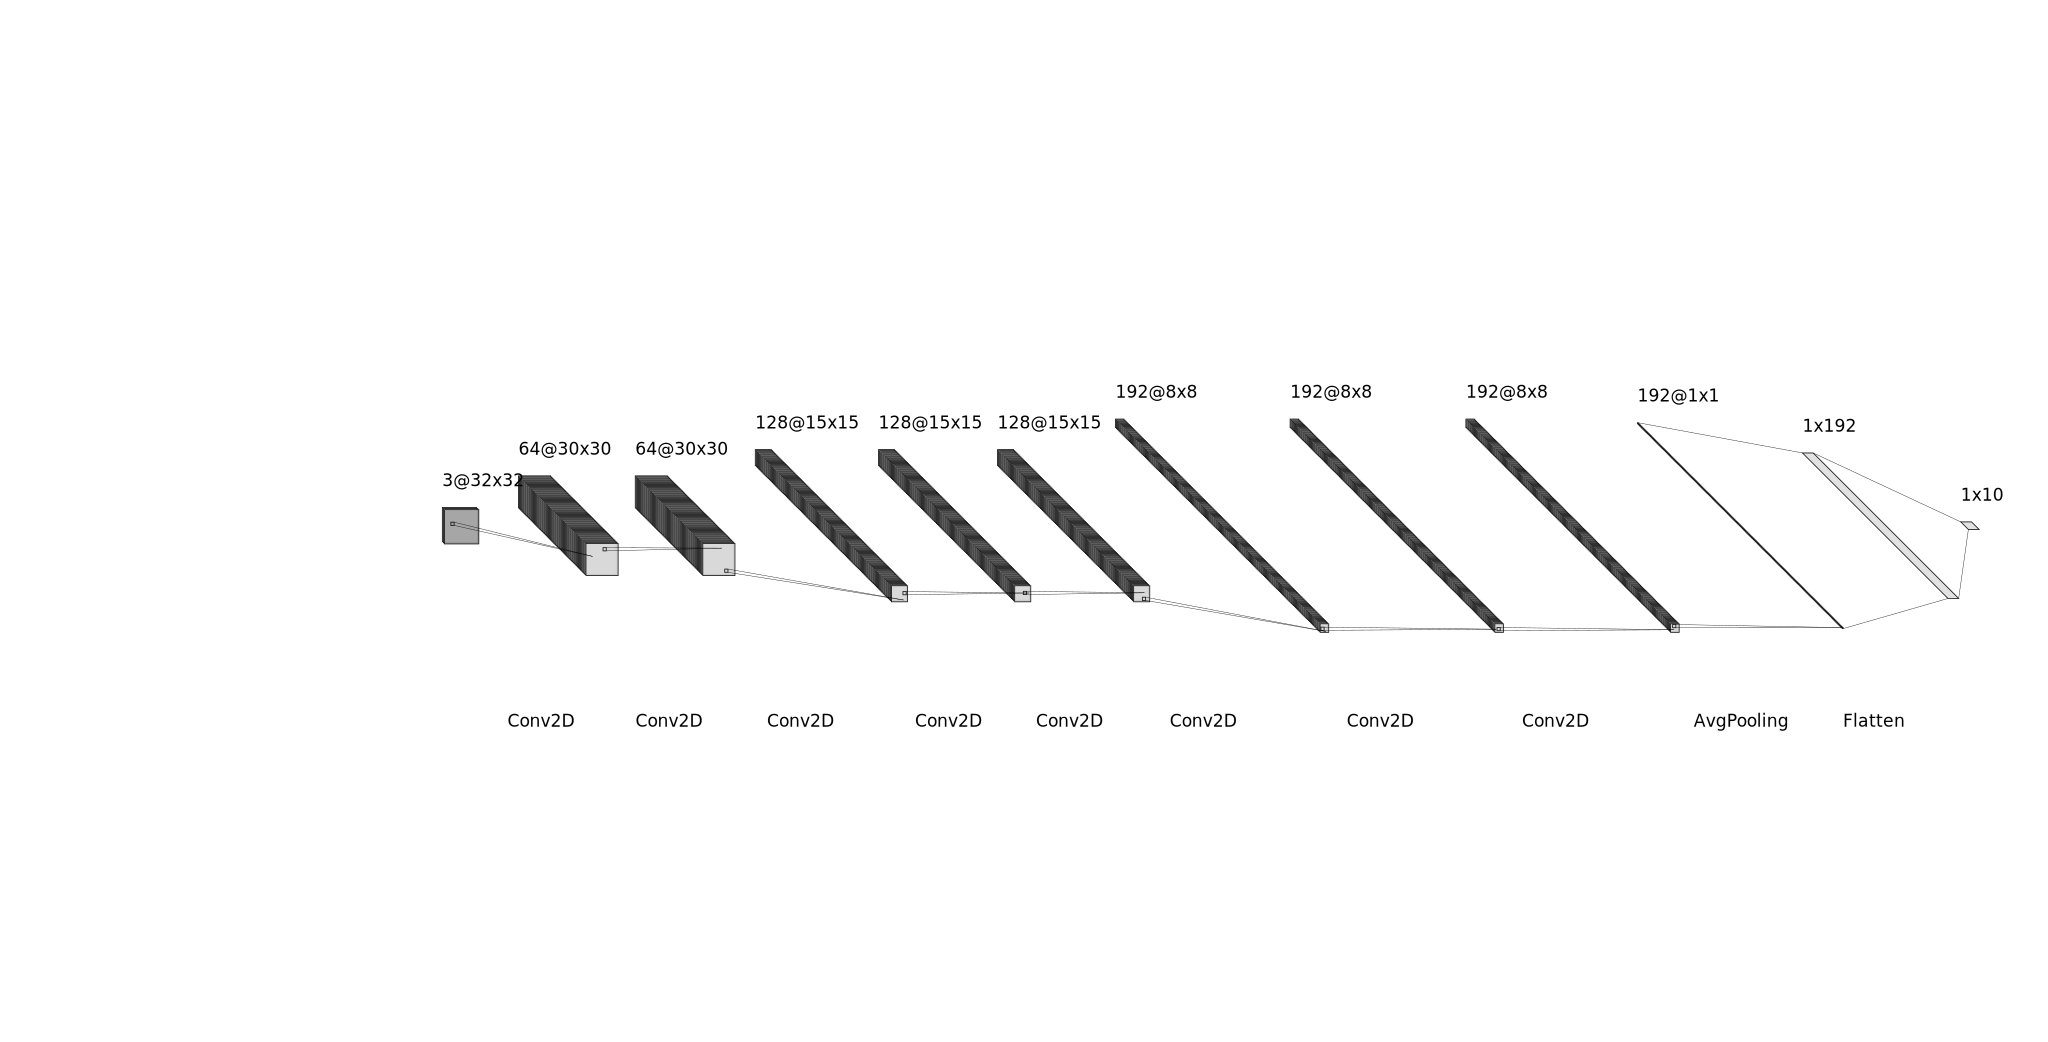
\includegraphics[scale=0.46]{Implementation/CFNArch.png}
    \caption{The Architecture of the CifarNet model}
    \label{fig:CFNArch}
\end{figure}

This was achieved by using Stochastic Gradient Descent as the optimizer and an adaptive learning rate and using a learning rate of $0.05$ for the first 50 epochs before shrinking it to $0.005$ for the next 25 epochs and finally $0.0005$ for the last 25. 
The face descriptor is then obtained in a similar manner to VGG where the softmax layer is taken out and the layer before is used as the face descriptor. 

\section{WGEML} \label{sec:WGEMLModule}

The main algorithm used in the project is Weighted Graph Embedding-Based Metric Learning (WGEML) \cite{WGEML}. The algorithm is a form of metric learning which takes in, as input, a training positive set for each face descriptor, $\mathcal{S}^p = \{(\mathbf{x}_i^p, \mathbf{y}_i^p) \mid 1 \leq i \leq N\}$ where $N$ is the number of image pairs in the set and a negative pair set $\mathcal{D}^p = \{(\mathbf{x}_i^p, \mathbf{y}_j^p) \mid 1 \leq i \leq N, j \neq i\}$. Let there be $M$ face descriptors for each image in the set. 
It also takes in a tuning parameter $r$ and a neighborhood size $K$ as input but those have been experimentally found to be 5 for each, each of which will be discussed later in this section. This section first gives an overview of the algorithm in Algorithm \ref{code:WGEMLPsuedocode} before discussing the problem statement in section \ref{sec:WGEMLProblem} and then the specifics of the approach in section \ref{sec:WGEMLApproach}. 

The overall algorithm is written in psuedocode in Algorithm \ref{code:WGEMLPsuedocode} from \cite{WGEML}.
\begin{algorithm}
\caption{WGEML}\label{code:WGEMLPsuedocode}
\textbf{Inputs}: The positive and negative pair sets $\mathcal{S}^p$ and $\mathcal{D}^p$ for each face descriptor, the tuning parameter $r$ and the number of neighbors to be considered $K$

\textbf{Outputs}: The matrices $\mathbf{U}_p$ and the weights $w_p$ for each face descriptor. 
\begin{algorithmic}[1]
\State Initialize $\mathbf{w}$
\State Initialize $\mathbf{U}$
\For{$p \in \{1, ..., M\}$}{}
    \State Use KNN to find the nearest neighbors of each $\mathbf{x}_i^p$ and $\mathbf{y}_i^p$. 
    \State Create the matrices $\mathbf{S}_p, \mathbf{D}_p, \mathbf{D}_{1p}, \mathbf{D}_{2p}$ using equations \ref{eqn:S_p}, \ref{eqn:D_p}, \ref{eqn:D_{1p}}, and \ref{eqn:D_{2p}}
    \State Regularize the matrix $\mathbf{S}_p$ using equation \ref{eqn:Regularize}
    \State Solve the eigenvalue problem in equation \ref{eqn:EigenvalueProblem} to get $\mathbf{U}_p$ and append it to $\mathbf{U}$
    \State Compute $w_p'$ using equation \ref{eqn:w_p'}and append it to $\mathbf{w}$
\EndFor
\State Divide each $w_p'$ in $\mathbf{w}$ by $\sum_{i = 1}^{M} w_p'$, as in equation \ref{eqn:Normalize}, to get the vector $\mathbf{w}$ such that the values sum to 1
\State Return $\mathbf{w}$ and $\mathbf{U}$. 
\end{algorithmic}
\end{algorithm}

\subsection{Problem} \label{sec:WGEMLProblem}

Given these inputs, the goal is to find the distance metrics and weights for:
\begin{align*}
d^2(\mathbf{x}_i, \mathbf{y}_i) &= \sum_{p = 1}^{M} w_p(\mathbf{x}_i^p - \mathbf{y}_i^p)^T\mathbf{A}_p(\mathbf{x}_i^p - \mathbf{y}_i^p)\\ 
&= \sum_{p = 1}^{M} w_p d^2_{\mathbf{A}_p}(\mathbf{x}_i^p, \mathbf{y}_j^p)
\end{align*}

Where $\mathbf{x}_i^p$ represents the $p$th face descriptor of the image $\mathbf{x}_i$, $w_p$ is a weight and $\mathbf{A}_p$ is a $D \times D$ semidefinite positive matrix, where $D$ is the dimensionality of the corresponding face descriptor. This distance function finds the distance between each pair of face descriptors and weights them accordingly.
We wish to find $\mathbf{A}_p$ such that the between-class variance is maximized, and the within-class variance is minimized. This can be formalized as the optimization problem:

\begin{align*}
    \max_{\mathbf{A}, \mathbf{w}} \mathcal{F} &= \sum_{p = 1}^{M} w_p^r[(\frac{1}{2}(\frac{1}{NK}\sum_{i = 1}^{N}\sum_{n_1 = 1}^{K} d^2_{\mathbf{A}_p}(\mathbf{x}_i^p, \mathbf{y}_{i,n_1}^p) + \frac{1}{NK}\sum_{i = 1}^{N}\sum_{n_2 = 1}^{K} d^2_{\mathbf{A}_p}(\mathbf{x}_{i,n_2}^p, \mathbf{y}_i^p)) \\
    & + \frac{1}{N} \sum_{i = 1, j \neq i}^{N} d^2_{\mathbf{A}_p}(\mathbf{x}_i^p, \mathbf{y}_j^p))/\frac{1}{N} \sum_{i = 1}^{N} d^2_{\mathbf{A}_p}(\mathbf{x}_i^p, \mathbf{y}_i^p)]
\end{align*}

\[\text{s.t. } \sum_{p = 1}^{M} w_p = 1\]
\[\forall p \in \{1, ..., M\}, w_p \geq 0\]
Where $\mathbf{y}_{i, n_1}^p$ is the $n_1$th nearest neighbor of $\mathbf{y}_i$ and similarly for $\mathbf{x}_{i, n_2}$. We have $w_p^r$ in order to avoid over-fitting and use information from each face descriptor. 
This optimization function tries to minimize the denominator which, in turn, pulls the samples that have the kin relationship together and maximizes the numerator which means that the pairs which don't have the kin relationship are pushed further away from each other as well as those of their neighbors.

\subsection{Approach} \label{sec:WGEMLApproach}

Now that the problem is defined, we break down $\mathbf{A}_p = \mathbf{U}_p\mathbf{U}_p^T$ since $\mathbf{A}_p$ is symmetric and positive semidefinite. $\mathbf{U}_p$ has size $D \times d$ such that $d \ll D$. In my project, $d$ was set to be $10$ by varying the value and seeing how it affects the accuracies and picking the best values.
Thus, the optimization problem can be rewritten as:

\[\max_{\mathbf{U}, \mathbf{w}}  \sum_{p = 1}^{M} w_p^r \frac{tr[\mathbf{U}_p^T(\frac{1}{2}(\mathbf{D}_{1p} + \mathbf{D}_{2p}) + \mathbf{D}_p)\mathbf{U}_p]}{tr[\mathbf{U}_p^T\mathbf{S}_p\mathbf{U}_p]}\]
Such that $\mathbf{U}_P^T \mathbf{U}_p = I$, $\sum_{p = 1}^{M} w_p = 1$ and $\forall p \in \{1, ..., M\}, w_p \geq 0$, where:

\begin{align} 
\mathbf{S}_p &= \frac{1}{N} \sum_{(\mathbf{x}_i^p, \mathbf{y}_i^p) \in \mathcal{S}^p} (\mathbf{x}_i^p - \mathbf{y}_i^p)(\mathbf{x}_i^p - \mathbf{y}_i^p)^T \label{eqn:S_p} \\
\mathbf{D}_p &= \frac{1}{N} \sum_{(\mathbf{x}_i^p, \mathbf{y}_j^p) \in \mathcal{D}^p} (\mathbf{x}_i^p - \mathbf{y}_j^p)(\mathbf{x}_i^p - \mathbf{y}_j^p)^T \label{eqn:D_p}\\
\mathbf{D}_{1p} &= \frac{1}{NK} \sum_{\substack{(\mathbf{x}_i^p, \mathbf{y}_i^p) \in \mathcal{S}^p \\ \mathbf{y}_k^p \in \mathcal{N}_K(\mathbf{y}_i^p)}} (\mathbf{x}_i^p - \mathbf{y}_k^p)(\mathbf{x}_i^p - \mathbf{y}_k^p)^T \label{eqn:D_{1p}}\\
\mathbf{D}_{2p} &= \frac{1}{NK} \sum_{\substack{(\mathbf{x}_i^p, \mathbf{y}_i^p) \in \mathcal{S}^p \\ \mathbf{x}_k^p \in \mathcal{N}_K(\mathbf{x}_i^p)}} (\mathbf{x}_k^p - \mathbf{y}_i^p)(\mathbf{x}_k^p - \mathbf{y}_i^p)^T \label{eqn:D_{2p}}
\end{align}

Where $\mathcal{N}_K(\mathbf{x}_i^p)$ represents the $K$ nearest neighbors of $\mathbf{x}_i^p$. This is when K-nearest neighbors is used, and $K$ is set to 5 in the experiments.
In order to solve this, we first let $\mathbf{w}$ be constant in order to solve $\mathbf{U}$ and then use that to find $\mathbf{w}$. By letting $\mathbf{w}$ be constant, the problem is reduced to:
\[\max_{\mathbf{U}_p^T \mathbf{U}_p = I} \frac{\text{tr}[\mathbf{U}_p^T(\frac{1}{2}(\mathbf{D}_{1p} + \mathbf{D}_{2p}) + \mathbf{D}_p)\mathbf{U}_p]}{\text{tr}[\mathbf{U}_p^T\mathbf{S}_p\mathbf{U}_p]}\]
For each $p \in \{1, ..., M\}$. This can then be converted to an alternative problem \cite{RatioTrace}:
\[\max_{\mathbf{U}_p}  \text{ tr}\left[(\mathbf{U}_p^T\mathbf{S}_p\mathbf{U}_p)^{-1} \mathbf{U}_p^T\paren*{\frac{1}{2}(\mathbf{D}_{1p} + \mathbf{D}_{2p}) + \mathbf{D}_p}\mathbf{U}_p\right]\]
Which can be solved by solving the following generalized eigenvalue problem:
\[\paren*{\frac{1}{2}(\mathbf{D}_{1p} + \mathbf{D}_{2p}) + \mathbf{D}_p}\mathbf{u} = \lambda \mathbf{S}_p \mathbf{u}\]
Thus, $\mathbf{U}_p = [u_1, u_2, ..., u_d]$ such that the corresponding eigenvalues for $u_1, .., u_d$ are the top $d$ largest eigenvalues (ie. $\lambda_1 \geq ... \geq \lambda_d$). However, this can be problematic in practice since $\mathbf{S}_p$ can be near singular when $D > N$. Thus, the identity matrix is added as a regularizer as follows:
\begin{equation}
\mathbf{S}_p = (1 - \beta)\mathbf{S}_p + \beta \frac{\text{tr}(\mathbf{S}_p)}{N}\mathbf{I} \label{eqn:Regularize}
\end{equation}
Where $\beta$ is a regularization parameter which is set to 0.5 experimentally. This allows us to then not need to solve the generalized eigenvalue problem, as that takes more computation time, and we can solve:

\begin{equation}
\mathbf{S}_p^{-1}\paren*{\frac{1}{2}(\mathbf{D}_{1p} + \mathbf{D}_{2p}) + \mathbf{D}_p}\mathbf{u} = \lambda \mathbf{u} \label{eqn:EigenvalueProblem}
\end{equation}
Thus, we have found $\mathbf{U}_p, \forall p \in \{1, ..., M\}$. 

To find the weights, $\mathbf{w}$, we can construct the Lagrangian:
\[\mathcal{L}(\mathbf{w}, \lambda) = \sum_{p = 1}^{M} w_p^r \frac{\text{tr}[\mathbf{U}_p^T(\frac{1}{2}(\mathbf{D}_{1p} + \mathbf{D}_{2p}) + \mathbf{D}_p)\mathbf{U}_p]}{\text{tr}[\mathbf{U}_p^T\mathbf{S}_p\mathbf{U}_p]} - \lambda \paren*{\sum_{p = 1}^{M}w_p - 1}\]
And thus, solve it:
\[\frac{\partial \mathcal{L}}{\partial w_p} = rw_p^{r-1} \frac{\text{tr}[\mathbf{U}_p^T(\frac{1}{2}(\mathbf{D}_{1p} + \mathbf{D}_{2p}) + \mathbf{D}_p)\mathbf{U}_p]}{\text{tr}[\mathbf{U}_p^T\mathbf{S}_p\mathbf{U}_p]} - \lambda = 0\]
\[\frac{\partial \mathcal{L}}{\partial \lambda} = \sum_{p = 1}^{M} w_p - 1 = 0\]
Which means:
\begin{equation}
w_p' = \paren*{\frac{\text{tr}[\mathbf{U}_p^T\mathbf{S}_p\mathbf{U}_p]}{\text{tr}[\mathbf{U}_p^T(\frac{1}{2}(\mathbf{D}_{1p} + \mathbf{D}_{2p}) + \mathbf{D}_p)\mathbf{U}_p]}}^{\frac{1}{r - 1}} \label{eqn:w_p'}
\end{equation}
\begin{equation}
w_p = \frac{w_p'}{\sum_{i = 1}^{M}w_i'} \label{eqn:Normalize}
\end{equation}
Thus, we now have the matrices to calculate the distance and the weights for each face descriptor. 

\section{Prediction} \label{sec:PredictionModule}

Given the matrices $U_p$ and weights $w_p$ from WGEML for all face descriptors where $U_p$ corresponds to the $p$'th face descriptor, we can use this to predict whether a given pair of images are of the kin relationship specified. 
First, we transform each of the faces into their $M$ face descriptors and use PCA to reduce the dimensions to the proper dimensionality. We then have $\mathbf{x} = \{x_p \mid 1 \leq p \leq M\}$ and $\mathbf{y} = \{y_p \mid 1 \leq p \leq M\}$.
Then, the similarity of these images can be calculated as follows, letting $A_p = U_pU_p^T$:

\[sim(\mathbf{x}, \mathbf{y}) = \sum_{p = 1}^{M} \frac{w_p}{2} \paren*{\frac{x_p^TA_py_p}{\sqrt{x_p^TA_px_p}\sqrt{y_p^TA_py_p}} + 1}\]

This ends up finding a weighted cosine similarity for a non-Euclidean space, since our metric here is $A_p$, for each face descriptor that is used. The function $sim$ ranges from $0$ to $1$ as needed of a similarity function. 
This differs from the version mentioned in \cite{WGEML} which was:
\[sim(\mathbf{x}, \mathbf{y}) = \sum_{p = 1}^{M} \frac{w_p}{2} \paren*{\frac{x_p^TU_p^TU_py_p}{\sqrt{x_p^TU_p^TU_px_p}\sqrt{y_p^TU_p^TU_py_p}} + 1}\]
However, as mentioned in section \ref{sec:WGEMLModule}, the model was trained such that $U_p^TU_p = I$ which would make this boil down to a weighted cosine similarity which wouldn't make much use of the metric learning. 
As such, this was changed up to use $A_p$ in the implementation rather than $U_p^TU_p$. 

In order to then determine whether two images are of the kin relationship specified, the similarity must then be compared to a threshold, $\theta$. If $sim(\mathbf{x}, \mathbf{y}) \geq \theta$, then the pair is labelled as having that relationship and, otherwise, it isn't.
As this value $\theta$ wasn't mentioned in \cite{WGEML}, it had to be found experimentally. By ranging over samples from $0$ to $1$, it was found that $\theta = 0.6$ yielded the best results for the accuracies and seemed the most similar to what the original paper had. 

\subsection{Tri-kin Relationship Prediction}

Due to the fact that tri-kin relationships have 3 images as the input, two parents and one child, the similarity is defined as the mean similarity between each of the parents and the child. In other words:

\[sim(\mathbf{p_1}, \mathbf{p_2}, \mathbf{c}) = \frac{sim(\mathbf{p_1}, \mathbf{c}) + sim(\mathbf{p_2}, \mathbf{c})}{2}\]

Where $\mathbf{p_1}, \mathbf{p_2}$ represent the face descriptors for each parent and $\mathbf{c}$ represents the face descriptors of the child.

\section{Overview of Workflow} \label{sec:Workflow}

There are 3 main stages to running the project, which are, for each dataset, the preprocessing stage, the training stage and then the testing stage. The important outputs of each of these stages are saved onto disk so that each stage doesn't have to be run right after another. 

\subsection{Preprocessing}

Given a dataset, we wish to precompute the face descriptors for each image and set up the 5-fold cross-validation for TSKinFace. The pipeline is shown in figure \ref{fig:PreprocessingPipeline}.

\begin{figure}[h!]
    \centering
    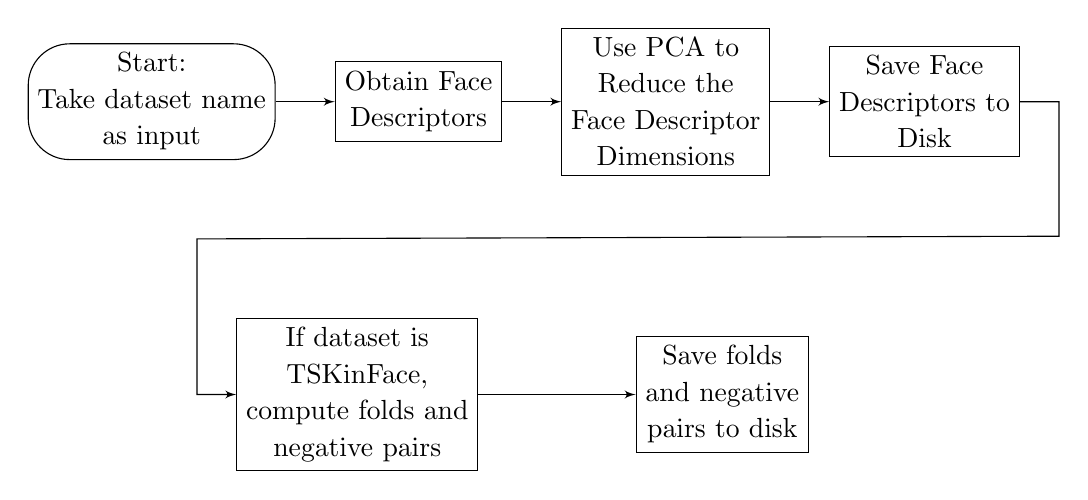
\begin{tikzpicture}[>=latex']
        \tikzset{block/.style= {draw, rectangle, align=center,minimum width=2cm,minimum height=1cm},
        rblock/.style={draw, shape=rectangle,rounded corners=1.5em,align=center,minimum width=2cm,minimum height=1cm},
        input/.style={ % requires library shapes.geometric
        draw,
        trapezium,
        trapezium left angle=60,
        trapezium right angle=120,
        minimum width=2cm,
        align=center,
        minimum height=1cm
    },
        }
        \node [rblock]  (start) {Start: \\ Take dataset name \\as input};
        \node [block, right =0.75cm of start] (FDs) {Obtain Face \\ Descriptors};
        \node [block, right =0.75cm of FDs] (PCA) {Use PCA to \\ Reduce the \\ Face Descriptor \\Dimensions};
        \node [block, right =0.75cm of PCA] (Save1) {Save Face \\ Descriptors to \\ Disk};
        \node [block, below right =2cm and -0.5cm of start] (TSKCV) {If dataset is \\ TSKinFace, \\ compute folds and \\ negative pairs};
        \node [block, right =2cm of TSKCV] (Save2) {Save folds \\ and negative \\ pairs to disk};
        \node [coordinate, below right =1cm and 0.5cm of Save1] (right) {};  %% Coordinate on right and middle
        \node [coordinate,above left =1cm and 0.5cm of TSKCV] (left) {};  %% Coordinate on left and middle

%% paths
        \path[draw,->] (start) edge (FDs)
                    (FDs) edge (PCA)
                    (PCA) edge (Save1)
                    (Save1.east) -| (right) -- (left)|- (TSKCV)
                    (TSKCV) edge (Save2)
                    ;
    \end{tikzpicture}

    \caption{The preprocessing pipeline}
    \label{fig:PreprocessingPipeline}
\end{figure}
\subsection{Training}

Once all of the face descriptors for each dataset are computed and, for each relationship in the dataset and for each setting (restricted or unrestricted), the cross-validation folds are created, the training set is properly made from the data and WGEML, which is described in section \ref{sec:WGEMLModule}, is run. The output of 
WGEML is then saved onto disk, which are the metrics and weights for each face descriptor for each fold. In the end, this is done for each relationship, setting and fold, so for KinFaceW-I, for example, there would be $4 \times 2 \times 5 = 40$ models saved. The pipeline is shown in figure \ref{fig:TrainingPipeline}.

\begin{figure}[h!]
    \centering
    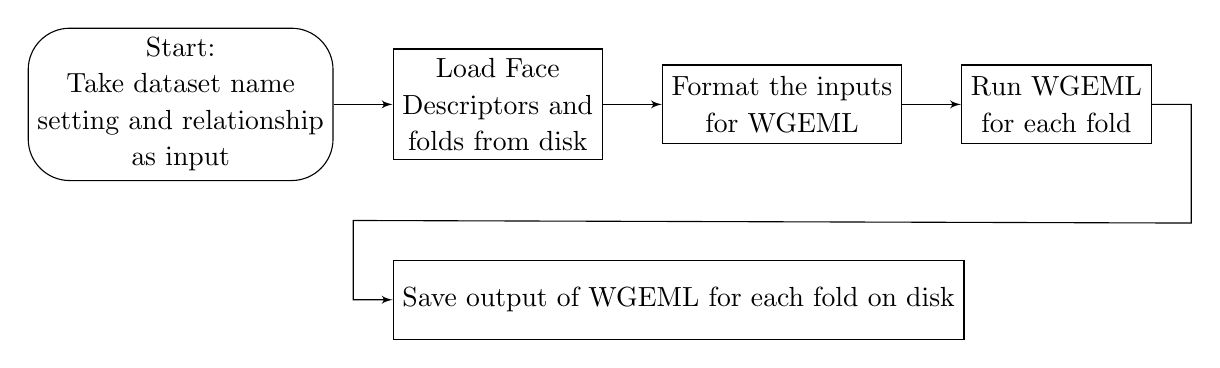
\begin{tikzpicture}[>=latex']
        \tikzset{block/.style= {draw, rectangle, align=center,minimum width=2cm,minimum height=1cm},
        rblock/.style={draw, shape=rectangle,rounded corners=1.5em,align=center,minimum width=2cm,minimum height=1cm},
        input/.style={ % requires library shapes.geometric
        draw,
        trapezium,
        trapezium left angle=60,
        trapezium right angle=120,
        minimum width=2cm,
        align=center,
        minimum height=1cm
    },
        }
        \node [rblock]  (start) {Start: \\ Take dataset name \\ setting and relationship \\as input};
        \node [block, right =0.75cm of start] (Load) {Load Face \\ Descriptors and \\ folds from disk};
        \node [block, right =0.75cm of Load] (Format) {Format the inputs \\ for WGEML};
        \node [block, right =0.75cm of Format] (WGEML) {Run WGEML \\ for each fold};
        \node [block, below right =1cm and 0.75cm of start] (Save) {Save output of WGEML for each fold on disk};
        \node [coordinate, below right =1cm and 0.5cm of WGEML] (right) {};  %% Coordinate on right and middle
        \node [coordinate, above left=0.5cm and 0.5cm of Save] (left) {};  %% Coordinate on left and middle

%% paths
        \path[draw,->] (start) edge (Load)
                    (Load) edge (Format)
                    (Format) edge (WGEML)
                    (WGEML.east) -| (right) -- (left)|- (Save)
                    ;
    \end{tikzpicture}
    \caption{The training pipeline}
    \label{fig:TrainingPipeline}
\end{figure}

\subsection{Testing}

Given a dataset, setting and relationship, the folds and the corresponding models are loaded from on disk, and, for each test set, the corresponding model is used to predict whether the images in the test set are of the given relationship or not. The accuracy is then recorded, and 
the average accuracy is outputted for the given configuration along with each of the individual accuracies, as shown in Figure \ref{fig:OutputOfTesting}. The pipeline is shown in figure \ref{fig:TestingPipeline}.

\begin{figure}[h!]
    \centering
    \includegraphics[scale=0.9]{Implementation/TrainingOutput.png}
    \caption{A sample output of the testing stage on KinFaceW-I unrestricted}
    \label{fig:OutputOfTesting}
\end{figure}

\begin{figure}[h!]
    \centering
    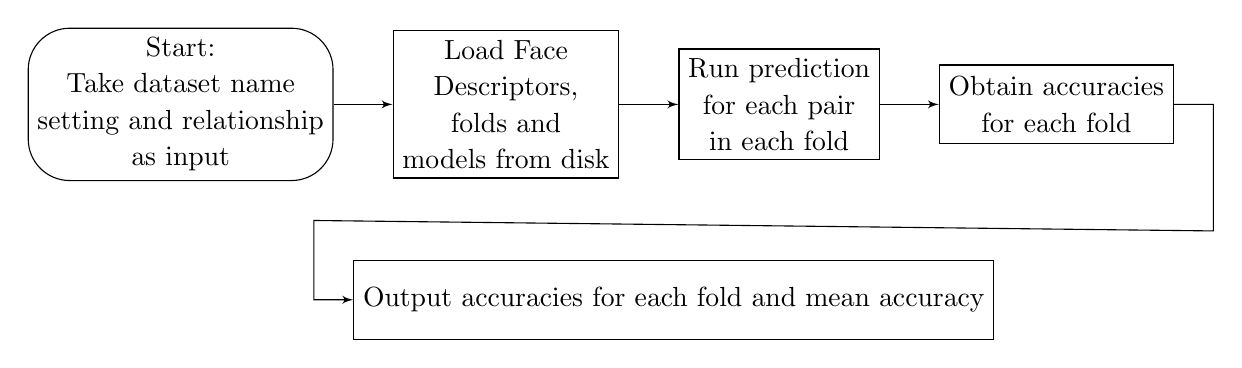
\begin{tikzpicture}[>=latex']
        \tikzset{block/.style= {draw, rectangle, align=center,minimum width=2cm,minimum height=1cm},
        rblock/.style={draw, shape=rectangle,rounded corners=1.5em,align=center,minimum width=2cm,minimum height=1cm},
        input/.style={ % requires library shapes.geometric
        draw,
        trapezium,
        trapezium left angle=60,
        trapezium right angle=120,
        minimum width=2cm,
        align=center,
        minimum height=1cm
    },
        }
        \node [rblock]  (start) {Start: \\ Take dataset name \\ setting and relationship \\as input};
        \node [block, right =0.75cm of start] (Load) {Load Face \\ Descriptors, \\ folds and \\ models from disk};
        \node [block, right =0.75cm of Load] (Predict) {Run prediction \\ for each pair \\ in each fold};
        \node [block, right =0.75cm of Predict] (Accs) {Obtain accuracies \\ for each fold};
        \node [block, below right =1cm and 0.25cm of start] (Out) {Output accuracies for each fold and mean accuracy};
        \node [coordinate, below right =1.1cm and 0.5cm of Accs] (right) {};  %% Coordinate on right and middle
        \node [coordinate, above left=0.5cm and 0.5cm of Out] (left) {};  %% Coordinate on left and middle

%% paths
        \path[draw,->] (start) edge (Load)
                    (Load) edge (Predict)
                    (Predict) edge (Accs)
                    (Accs.east) -| (right) -- (left)|- (Out)
                    ;
    \end{tikzpicture}

    \caption{The testing pipeline}
    \label{fig:TestingPipeline}
\end{figure}

%%%%%%%%%%%%%%%%%%%%%%%%%%%%%%%%%%
%%%%%%%%%%% Evaluation %%%%%%%%%%%
%%%%%%%%%%%%%%%%%%%%%%%%%%%%%%%%%%


\chapter{Evaluation} \label{chapter:Evaluation}

In this chapter, I will discuss the accuracies that were obtained from the project in section \ref{sec:MainResults} whether the success criterion was achieved in section \ref{sec:SuccCriterionEval}. 
Then, the potential biases in these datasets are discussed in section \ref{sec:Biases}, the ablation studies are discussed in section \ref{sec:AbStudies}, the CifarNet extension results will be discussed in section \ref{sec:CFNResults} and finally the unit tests and their coverage will be briefly discussed in section \ref{sec:UnitTests}. 

\section{Overall Accuracies of the Model} \label{sec:MainResults}

As mentioned in section \ref{sec:Datasets}, we have that ``F'' stands for father, ``M'' stands for mother, ``S'' stands for son, and ``D'' stands for daughter so the relationships are noted as a combination of these acronyms, so ``FS'' stands for the Father-Son relationship, etc. The project is run end-to-end for each dataset, setting and relationship and the accuracies are shown in figure \ref{fig:Accs}. For the success criterion, we look at the difference between the accuracies my implementation had obtained, and the original paper had obtained, which is shown in figure \ref{fig:diffInAccs} where a positive number means my accuracies were better. 

\begin{figure}[h!]
    \centering
    \includegraphics[scale=0.68]{Eval/OrigResults.png}
    \caption{Accuracies of WGEML applied to each dataset for each relationship grouped by dataset}
    \label{fig:Accs}
\end{figure}

\begin{figure}[h!]
    \centering
    \includegraphics[scale=0.65]{Eval/DiffOrigResults.png}
    \caption{Differences in accuracies between my implementation and \cite{WGEML} in \%}
    \label{fig:diffInAccs}
\end{figure}

We can see that none of the absolute values of the differences go higher than $8.89\%$ which, as will be discussed in \ref{sec:SuccCriterionEval}, means that the success criterion is fulfilled. 

% We also see that the Father-Son relationship does better than the other relationships for the same dataset except in the Mother-Son relationship for TSKinFace when there were only positive pairs in the training set and both positive and negative pairs in the testing set. 
In general, we see that the accuracies of the Father-Son relationship for each dataset are higher than those of the other relationships. However, there is one exception to this which is in the TSKinFace dataset when we use only positive pairs in the training set and both positive and negative pairs in the testing set.

When only positive pairs were used for the TSKinFace dataset for both training and testing, we get accuracies that are fairly close to that of the original paper with an average difference of $0.742\%$. However, when negative pairs were added to the test set, the accuracies drop by, on average, $8.29\%$. This led me to believe that the original paper had only used the positive pairs for the testing phase of TSKinFace as TSKinFace didn't come with any premade negative pairs. As a note, in the later sections of this chapter, TSKinFace refers to having all pairs in both the training and test set. 

\section{Success Criterion} \label{sec:SuccCriterionEval}

As seen in section \ref{sec:MainResults}, I was able to replicate the accuracies from \cite{WGEML} within a $\pm 15\%$ accuracy by using the WGEML methodology which means that the project is a success according to appendix \ref{chapter:Proposal}. 
% Furthermore, referring to the requirements analysis in section \ref{sec:ReqAnal}, each of the core project requirements were completed, which were to implement face detection, the necessary face descriptors, WGEML, a prediction method and replicate the paper end-to-end. 
Furthermore, the extensions were also completed and the results of which are discussed in sections \ref{sec:Biases}, \ref{sec:AbStudies}, and \ref{sec:CFNResults}.

\section{Receiver Operating Characteristic (ROC) Curves}

We can also examine the ROC curves for each dataset in figure \ref{fig:ROCCurves}.

\begin{figure}[h!]
    \centering
    \includegraphics[scale=0.6]{Eval/ROC.png}
    \caption{The mean ROC curve for each dataset averaged over each fold, relationship and setting}
    \label{fig:ROCCurves}
\end{figure}

Here, we see that the area under the curve is the most for the TSKinFace dataset and the least for the KinFaceW-I dataset, though both curves are far from that of a classifier that is luck-based. 

\section{Potential Biases in Datasets} \label{sec:Biases}

In order to look at potential biases that could occur in each of the datasets, each model was tested on all of the datasets that were available. So, for example, the model that was returned from training on the KinFaceW-I unrestricted dataset for the Father-Son relationship will have been tested on all of the 3 datasets that were used. 

In every case, the accuracies went down when the test set that was used came from a different dataset than the training set. This is to be expected as the model might be overfitting to small biases that are inherent in every dataset. 
The models trained with the KinFaceW-I dataset generalizes fairly well, compared to KinFaceW-II and TSKinFace, since it seems to have the lowest differences of the 3 datasets 
with an average of an 8\% decrease in accuracy compared to the accuracies when it is tested with itself. 
Then, KinFaceW-II was worse at a difference of 11.7\% and then TSKinFace was by far the worst with an 
average difference of 15.7\%. The average accuracy difference across the two test datasets for each training dataset and relationship is shown in figure \ref{fig:PairwiseAccByRel} and the average accuracy differences for each dataset across all relationships and test datasets is shown in figure \ref{fig:AvgPairwiseAcc}.

\begin{figure}[h!]
    \centering
    \includegraphics[scale=0.6]{Eval/AvgPairwiseAccByRelationship.png}
    \caption{The average accuracy differences of the two test datasets for each training dataset and relationship}
    \label{fig:PairwiseAccByRel}
\end{figure}
 
\begin{figure}[h!]
    \centering
    \includegraphics[scale=0.6]{Eval/AvgPairwiseAcc.png}
    \caption{The average accuracy differences of the two test datasets and relationship for each training dataset}
    \label{fig:AvgPairwiseAcc}
\end{figure}

The main reason for this is due to the fact that both KinFaceW-II 
and TSKinFace get the positive pairs from the same image whereas KinFaceW-I doesn't. 
At a high-level view, this means that WGEML might be taking into account the lighting of the image or other 
non-face related features of the image and WGEML is using the similarity of those features more in the 
KinFaceW-II and TSKinFace datasets than actual facial features. This means that WGEML might be picking up on these cues in order to increase performance \cite{dawson2018photo}. 
For example, if a pair of images that have a similar lighting comes up, at a high-level, WGEML might be using the fact that it has similar lighting to infer that the faces come from the same photo and thus are more likely to be related. 
Since pairs in KinFaceW-I aren't from the same image, necessarily, WGEML is able to generalize better which explains why the differences are smaller than 
that of KinFaceW-II and TSKinFace. 

\section{Ablation Studies} \label{sec:AbStudies}

\subsection{Blocking Face Descriptors} \label{sec:FDAbStudies}

Ablation studies were done by using each possible subset of the $4$ face descriptors that were originally used for WGEML for training and testing. For example, only the VGG face descriptor was used for training and testing and the accuracies were obtained for each dataset, setting, and relationship.

After obtaining each accuracy for each dataset, setting, relationship and subset of face descriptors, I decided to group up the accuracies by the amount of face descriptors used by averaging the accuracies for each subset of that number.

As expected, in general, as the number of face descriptors are increased, the accuracy increases as well. 
However, as you increase the number of face descriptors, there are diminishing returns on the accuracy (ie. the second derivative is negative). An example of this is shown with KinFaceW-II unrestricted which is shown in figure \ref{fig:AbStudy}.

\begin{figure}[h!]
    \centering
    \includegraphics[scale=0.6]{Eval/AbStudy.png}
    \caption{The plot of accuracy versus number of face descriptors used for each unrestricted dataset}
    \label{fig:AbStudy}
\end{figure}

The only dataset this doesn't seem to apply to is KinFaceW-I unrestricted in which adding a second 
face descriptor increases the accuracy quite a bit but the third doesn't increase it too much and then the fourth 
increases it more, as seen in figure \ref{fig:AbStudy}.

However, this is mainly due to two outliers, for the FD relationship, 
increasing from 2 to 3 face descriptors only increased the accuracy by 0.2\% and for the MS relationship, 
going from 3 to 4 increased accuracy by 3\%.  % Would showing the raw numbers be good here?
 
At a high-level, as more face descriptors are added, the features 
that each face descriptor capture are more likely to overlap with each other, compared to when 
there's only one face descriptor, in which case another one could add a lot more information. 
However, if there are already 3 face descriptors, another face descriptor might share a lot of 
the same information the others already have captured and only be able to add, relatively, 
a small amount of information.

I then looked at which individual configurations of face descriptors used, and relationship resulted in a 
better accuracy than if all of the face descriptors were used.
One thing I saw was that, out of the 22 instances this happened among all of the datasets, 
all of them used the VGG face descriptor.
This led me to believe that the VGG descriptor is quite useful when used in conjunction 
with at least one other face descriptor, since we also had that the configurations that 
used VGG tended to do better in accuracy than the ones that didn't, from what I could see. 
This makes sense since VGG is a deep feature detector whereas the other face descriptors use the texture only.
 
Furthermore, the KinFaceW-I restricted configuration had by far the 
highest number of configurations which did better than using all 4 face descriptors for that 
relationship, with 11 of the 22 configurations. The other datasets had about 3-4 instances where 
this occurred. 


\section{CifarNet Extension} \label{sec:CFNResults}

When I replaced VGG with CifarNet (CFN), I found that it does worse in the KinFaceW-I dataset, 
it does better in the KinFaceW-II dataset, and it doesn't have a huge effect on the TSKinFace dataset 
(with the biggest difference being a 1\% difference in accuracy). When grouped by relationship, I 
found that the father-son relationship had the least change in accuracy with an average 0.092\% 
accuracy difference. This is shown in figure \ref{fig:CFNRelationshipGrouping} where a positive number implies that the original face descriptors did better. There is more variation in the other relationships than there is in the father-son relationship, 
and this is reflected in the standard deviations for each relationship, ignoring the tri-kin relationships as there is only one dataset for this. 

The differences grouped by dataset is shown in figure \ref{fig:CFNDatasetGrouping}.

\begin{figure}[h!]
    \centering
    \includegraphics[scale=0.6]{Eval/DiffAccCFNRelationship.png}
    \caption{Differences in accuracy when VGG is replaced with CFN grouped by relationship}
    \label{fig:CFNRelationshipGrouping}
\end{figure}
 
\begin{figure}[h!]
    \centering
    \includegraphics[scale=0.6]{Eval/DiffAccCFNDataset.png}
    \caption{Differences in accuracy when VGG is replaced with CFN grouped by dataset}
    \label{fig:CFNDatasetGrouping}
\end{figure}

In general, VGG did better than CFN for KinFaceW-I and did worse for KinFaceW-II. 
The maximum difference in accuracies was 5.4\% which occurred in the KinFaceW-II unrestricted setting with 
the mother-daughter relationship in which CFN made the accuracy increase by 5.4\%. The maximum decrease 
in accuracy was 4.7\% with the KinFaceW-I Restricted dataset for the mother-son relationship. The KinFaceW-II 
Unrestricted setting with the mother-son relationship had no difference whatsoever in accuracies between the 
face descriptors. 

Although VGG generally did better accuracy-wise, it might be useful to use the CFN descriptor instead due to the smaller model which means that there is less computation when it comes to prediction. The fact that it is a smaller model also means that there are less weights so the file the weights are saved to is smaller, which can be seen since the CFN weights are 5MB whereas the VGG weights are 566MB. 
This means that using the CFN model can be useful in mobile and embedded systems whereas having the extra computation and size cost might not be worth it for the $5\%$ gain in some cases. 

\section{Unit Tests} \label{sec:UnitTests}

To make sure the project was doing everything that it was supposed to be doing, unit tests were created for each file except the scripts due to the fact that the scripts were for integrating the modules together and thus didn't require unit testing.
The statement coverage for each file and overall is shown in figure \ref{fig:Coverage}. In general, most of the files had 100\% statement coverage and the main reason that CifarNet doesn't have a higher coverage is due to a function which trains the model and another function which packages up the creation of the model and training the model into one function. This is fairly difficult to unit test from my knowledge, which is what makes up the most of the untested code.

\begin{figure}[h!]
    \centering
    \includegraphics{Eval/Coverage.png}
    \caption{Coverage of the unit tests of the project}
    \label{fig:Coverage}
\end{figure}

%%%%%%%%%%%%%%%%%%%%%%%%%%%%%%%%%%
%%%%%%%%%%% Conclusion %%%%%%%%%%%
%%%%%%%%%%%%%%%%%%%%%%%%%%%%%%%%%%

\chapter{Conclusion}

Overall, the project was successful since I was able to replicate implement each of the core components, as specified in section \ref{sec:ReqAnal} and, this allowed me to replicate the findings of the WGEML paper within a 15\% error range. 
Furthermore, I was able to further explore the intricacies of the algorithm and how it reacts to variations in the input. By doing ablation studies, 
I was able to discover that adding face descriptors to the algorithm has diminishing returns in section \ref{sec:FDAbStudies}. Furthermore, sources of bias in the datasets were found in section \ref{sec:Biases}.

\section{Lessons Learnt}

One of the main lessons I learnt was with respect to how important testing is. By writing these unit tests, even for seemingly simple functions, I saved myself a lot of potential future problems as I was able to catch many of the bugs while I was writing the code instead of at the integration stage. Of course, there were still bugs when I tried running the project end-to-end, but these were much simpler to solve knowing that each individual function I wrote and used is correct. 
For example, solving the eigenvalue problem and getting the top $d$ vectors with respect to WGEML is a fairly simple function to write. However, had I not created some non-trivial matrices to test that function with, I wouldn't have realized that the function was only returning $d$ elements of each eigenvector instead of $d$ eigenvectors. 

As I hadn't had much experience with Computer Vision prior to this project, a lot of research had to be done into the intricacies of the original WGEML paper, such as what each face descriptor is and how they work. I was able to learn how to read multiple research papers and consolidate their information into my project. 

Dependencies posed minor problems at points. Although I had a \texttt{requirements.txt} file and a virtual environment, running the testing pipeline on my laptop caused different results to the external GPU I was using for running the project end-to-end. The testing pipeline was the only pipeline I could reasonably run on my laptop due to its simplicity. However, 
due to the fact that I had changed some of the dependencies in the \texttt{requirements.txt} file on the external GPU, I had obtained different results. I realized how important maintaining the same dependencies was to a project.

If I were to do the project over again, I think using more sophisticated software engineering tools such as some continuous integration tool such as Jenkins together with a containerization tool such as Docker would help immensely. Sometimes I would forget to run my unit tests before pushing my changes to the feature branch and only afterwards I would realize that the unit tests fail and one time I only noticed after the broken changes had already reached the master branch which continuous integration could help prevent. Docker could have also helped to prevent the dependency issue I had. 

\section{Future Work}

In the future, the model can be extended to work on videos. This was an extension at the beginning of the project which ended up not coming to fruition due to the fact that I couldn't obtain a dataset for it.  
Furthermore, the project can be extended such that the potential relationship doesn't have to be specified in the input, which would answer whether two people are related at all rather than if they are related in a specific way. 

Aside from extensions regarding the implementation, we can also further explore whether, in the ablation studies, the graph of accuracy versus the number of face descriptors continues in the way I'd expect with it leveling off after enough face descriptors or does it go down after a bit since the abundance of information could potentially interfere with each other? Furthermore, how would the different sets of face descriptors used affect this?
Furthermore, in the original results, there wasn't much difference in accuracies between the unrestricted and restricted settings in many of the cases. In this case, the effect the negative pairs has on the algorithm can be further explored and whether different sets of negative pairs can give statistically significant differences in the accuracies. 

%%%%%%%%%%%%%%%%%%%%%%%%%%%%%%%%%%%%%%%%%%%%%%%%%%%%%%%%%%%%%%%%%%%%%
% the bibliography
\addcontentsline{toc}{chapter}{Bibliography}
\bibliographystyle{plain}
\bibliography{citations.bib}

%%%%%%%%%%%%%%%%%%%%%%%%%%%%%%%%%%%%%%%%%%%%%%%%%%%%%%%%%%%%%%%%%%%%%
% the appendices
\appendix

\chapter{Algorithms Implemented in Libraries} 

\section{Cascade Classifier} \label{sec:Cascade}

\section{SIFT Keypoint Extraction} \label{sec:AppendixSIFT}

The first thing to do is to create octaves for the given image. An octave is a set of the given image being blurred multiple times. 
For example, in the first octave, the original image is the first image, and then the next image is blurred slightly which is then blurred further for the next image in the octave, etc. In the second octave, the image is halved in size and the same blurring effect happens. So, if the original image was of size $64 \times 64$, then the images in the second octave will be $32 \times 32$ and in the third it would be $16 \times 16$ and so on. A specified number of octaves and blurred images are used for the SIFT algorithm. The way that the image is blurred is as follows:
\[L(x, y, \sigma) = G(x, y, \sigma) * I(x, y)\]
Where $x, y$ is the coordinate in the image, $I$ is the function mapping coordinates to the value of the image at that coordinate, $\sigma$ is the amount of blurring, $*$ represents convolving $G$ on the image and:
\[G(x, y, \sigma) = \frac{1}{2\pi\sigma^2}e^{-\frac{x^2 + y^2}{2\sigma^2}}\]
Which is the Gaussian blur. 

From here, for each octave, a difference of Gaussians is created to help find the keypoints of the image. The difference of Gaussians is just the difference between the consecutive Gaussians. This can be visualized in figure \ref{fig:DiffOfGauss}.

\begin{figure}[ht]
    \centering
    \includegraphics[scale=0.2]{Prep/DoG.png}
    \caption{The Difference of Gaussians being created. Image reproduced from Lowe (2004) \cite{SIFT}}
    \label{fig:DiffOfGauss}

\end{figure}

This is used to approximate the Laplacian of Gaussians as the LoG helps find the edges of the image by blurring the image a bit and then finding the second order derivatives. It is first blurred as taking the Laplacian straight away would be sensitive to noise. However, this is computationally expensive. The Difference of Gaussians is a good approximation of the scale invariant Laplacian, $\sigma^2\nabla^2G$.

From here we look for the keypoints in the image using the Difference of Gaussians. This is done by finding the local maxima and minima of the DoG. Once the extrema of the Difference of Gaussians are obtained, we need to refine the approximation of the keypoint because the actual keypoint is more likely to be between pixels. Thus, we can use a Taylor expansion around the proposed keypoint of the scale-space function $D(\sigma, x, y)$ where $\sigma$ is the blur level in the DoG. This Taylor expansion looks like:
\[D(\mathbf{x}) = D + \frac{\partial D}{\partial \mathbf{x}}^T\mathbf{x} + \frac{1}{2}\mathbf{x^T}\frac{\partial^2 D}{\partial \mathbf{x}^2}\mathbf{x}\]
Where $D$ is the value of $D$ at the proposed keypoint, $\mathbf{x} = (\sigma, x, y)^T$, $\frac{\partial D}{\partial \mathbf{x}}^T = (\frac{\partial D}{\partial \sigma}, \frac{\partial D}{\partial x}, \frac{\partial D}{\partial y})$. Letting this equal 0, we get that the offset from our keypoint is:
\[\hat{\mathbf{x}} = - \frac{\partial^2 D}{\partial \mathbf{x}^2}^{-1} \frac{\partial D}{\partial \mathbf{x}}\]
If our offset is greater than 0.5 in any dimension, then we want to try again since that means it's closer to another sample point. We keep trying again until we get an offset which is close to the sample point. We then find the value at the subpixel extrema:
\[D(\hat{\mathbf{x}}) = D + \frac{1}{2}\frac{\partial D}{\partial \mathbf{x}}^T\hat{\mathbf{x}}\]
And if the value of the extrema is less than $0.03 \times 255$, then we throw it out since it is an unstable extrema and has low contrast. 

Furthermore, we also eliminate any keypoints that are potentially on an edge. We can do this by looking at the Hessian of the keypoint. We have that the Hessian is:
\[\mathbf{H} = \begin{bmatrix}
        D_{xx} & D_{xy}\\
        D_{yx} & D_{yy}
    \end{bmatrix}\]
To determine whether something is a corner, we care about the eigenvalues of $\mathbf{H}$, or more specifically, the ratio between the eigenvalues. Using the trace and determinant of $\mathbf{H}$, we can find that:
\[\frac{\text{Tr}(\mathbf{H})^2}{\text{Det}(\mathbf{H})} = \frac{(r+1)^2}{r}\]
Where $r$ is the ratio of the eigenvalues. Thus, letting the maximum ratio that the eigenvalues are allowed to be at be $r_0 = 10$, we just need to find if:
\[\frac{\text{Tr}(\mathbf{H})^2}{\text{Det}(\mathbf{H})} < \frac{(r_0+1)^2}{r_0}\]
If it is, then this is a proper keypoint. If it isn't then this is an edge so we can discard it. 

We now have each of the keypoints which are scale-invariant, so we need to make it rotation-invariant as well. This is done by assigning an orientation to the keypoints. A neighborhood is taken around the keypoint in which the gradient is obtained for each pixel in the area and a histogram of these gradients is created based on the angle, this time in bins of $0$ to $10$, 10 to 20, etc. until 350 to 360. The peak in this histogram is calculated and taken and any other peaks which have a value above 80\% of the original peak is also considered to calculate the orientation. Now, for each keypoint, we have the location, scale, and orientation.

\section{Principal Component Analysis} \label{sec:PCA}

Principal Component Analysis (PCA) \cite{PCA} is a statistical tool that we can use to reduce the dimensionality of a dataset while maintaining as much of the variability as possible. The algorithm identifies \textit{principal components} which are the directions of maximum variance in the dataset, which can be visualized in figure \ref{fig:PCA}.

\begin{figure}[ht]
    \centering
    \includegraphics[scale=0.5]{Prep/PCAComps.jpeg}
    \caption{Principal components of an arbitrary 2 dimensional dataset}
    \label{fig:PCA}
\end{figure}

Let $p$ be the number of variables that are being measured in the dataset, which in our case is the dimension of the face descriptor. Let $\mathbf{X}$ be the matrix $n \times p$ data matrix that is composed of the $p$ $n$-dimensional vectors $\mathbf{x_1}, ..., \mathbf{x_p}$ in which $x_i$ represents the $n$ observations of the $i$th variable.
The goal of PCA is then to create a $p \times k$ matrix $\mathbf{W}$, where $k \leq p$, which maps each row-vector of $\mathbf{X}$ from the original $p$-dimensional feature space to a new $k$-dimensional feature subspace such that the variability of the dataset is kept intact, as much as possible. 

First, the dataset must be standardized which means that the mean of each feature must be $0$, which we denote as the matrix $\mathbf{X'}$ and the column vectors as $\mathbf{x_1'}, ..., \mathbf{x_p'}$. From there, the covariance matrix is obtained. This matrix is the following:

\[\Sigma = \begin{bmatrix}
    Cov(\mathbf{x_1'}, \mathbf{x_1'}) & ... & Cov(\mathbf{x_1'}, \mathbf{x_p'}) \\
    \vdots & \ddots & \vdots \\
    Cov(\mathbf{x_p'}, \mathbf{x_1'}) & ... & Cov(\mathbf{x_p'}, \mathbf{x_p'})
\end{bmatrix}\]

Where:

\[\Sigma_{ij} = Cov(\mathbf{x_i'}, \mathbf{x_j'}) = \frac{1}{n}(\mathbf{x_i'}\cdot \mathbf{x_j'})\]

Since we have that the mean of both are $0$ now, after standardization. Thus:

\[\Sigma = \frac{1}{N} \mathbf{X'}\mathbf{X'}^T\]

We then find the eigenvalues and eigenvectors of $\Sigma$, of which we get $p$ of them. The eigenvalues get sorted from largest to smallest and, thus, the first principal component is the eigenvector that corresponds to the largest eigenvalue, the second principal component is the eigenvector with the second largest eigenvalue, etc. 
Denoting $\mathbf{w_i}$ as the $i$th principal component, we can make the matrix $\mathbf{W}$ as:

\[\mathbf{W} = \begin{bmatrix}
    \mathbf{w_1} & ... & \mathbf{w_k}
\end{bmatrix}\]

Which is a $p \times k$ matrix. Thus, to reduce the dimensions of the original dataset, we can create the matrix:

\[\mathbf{T} = \mathbf{X}\mathbf{W}\]

In which the $i$th row of $\mathbf{T}$ corresponds with the $i$th observation of $\mathbf{X}$ and this vector has is $k$-dimensional where $k \leq p$. 


\chapter{Raw Table Data}

The tables for figures \ref{fig:Accs} and \ref{fig:diffInAccs} is as follows:

\begin{table}[h!]
\centering
\begin{tabular}{c|c|c|c|c|c|c|c}
    Dataset & Setting                       & FS     & FD     & MS     & MD     & FMS    & FMD    \\\hline
    KFWI    & Unrestricted                  & 0.8015 & 0.7166 & 0.7628 & 0.7921 &        &        \\
    KFWI    & Restricted                    & 0.811  & 0.7391 & 0.7405 & 0.769  &        &        \\
    KFWII   & Unrestricted                  & 0.838  & 0.778  & 0.832  & 0.78   &        &        \\
    KFWII   & Restricted                    & 0.848  & 0.768  & 0.802  & 0.814  &        &        \\
    TSK     & Only Positive Pairs           & 0.9201 & 0.8826 & 0.9162 & 0.9182 & 0.9571 & 0.9343 \\
    TSK     & All Pairs In Test/Pos Pairs in Train      & 0.8409 & 0.8282 & 0.8448 & 0.8193 & 0.8566 & 0.86   \\
    TSK     & All Pairs In Test/Train             & 0.8409 & 0.8203 & 0.8242 & 0.8362 & 0.8664 & 0.8431
\end{tabular}
\caption{Accuracies of WGEML applied to each dataset for each relationship}
\label{table:Accs}
\end{table} 

\begin{table}[h!]
\centering
\begin{tabular}{c|c|c|c|c|c|c|c}
    Dataset & Setting                  & FS    & FD    & MS    & MD    & FMS   & FMD   \\\hline
    KFWI    & Unrestricted             & 1.65  & -2.24 & -4.32 & -2.69 &       &       \\
    KFWI    & Restricted               & 2.2   & 0.71  & -5.35 & -3.8  &       &       \\
    KFWII   & Unrestricted             & -4.8  & 0.4   & -0.2  & -3.6  &       &       \\
    KFWII   & Restricted               & -3.4  & -0.6  & -3    & -1    &       &       \\
    TSK     & Only Positive Pairs      & 1.71  & -1.54 & 0.22  & 1.42  & \textbf{2.21}  & 0.43  \\
    TSK     & All Pairs In Test/Pos Pairs in Train & -6.21 & -6.98 & -6.92 & -8.47 & -7.84 & -7    \\
    TSK     & All Pairs In Test/Train        & -6.21 & -7.77 & \textbf{-8.98} & -6.78 & -6.86 & -8.69
\end{tabular}
\caption{Differences in accuracies between my implementation and \cite{WGEML} in \%}
\label{table:diffInAccs}
\end{table}    

\chapter{Sample Code}

\chapter{Project Proposal}\label{chapter:Proposal}

% \input{Proposal/proposal}

\end{document}